%% The following is a directive for TeXShop to indicate the main file
%%!TEX root = diss.tex
\chapter{Supporting Materials}

This would be any supporting material not central to the dissertation.
For example:
\begin{itemize}
\item radiometry
\item technical details of MVS, PS, SL, SfS, etc
\end{itemize}

\section{Material of real-world objects}
\begin{table}[!hbtp]
  \centering
  \begin{tabular}{*{9}{c}}
  \multicolumn{3}{l}{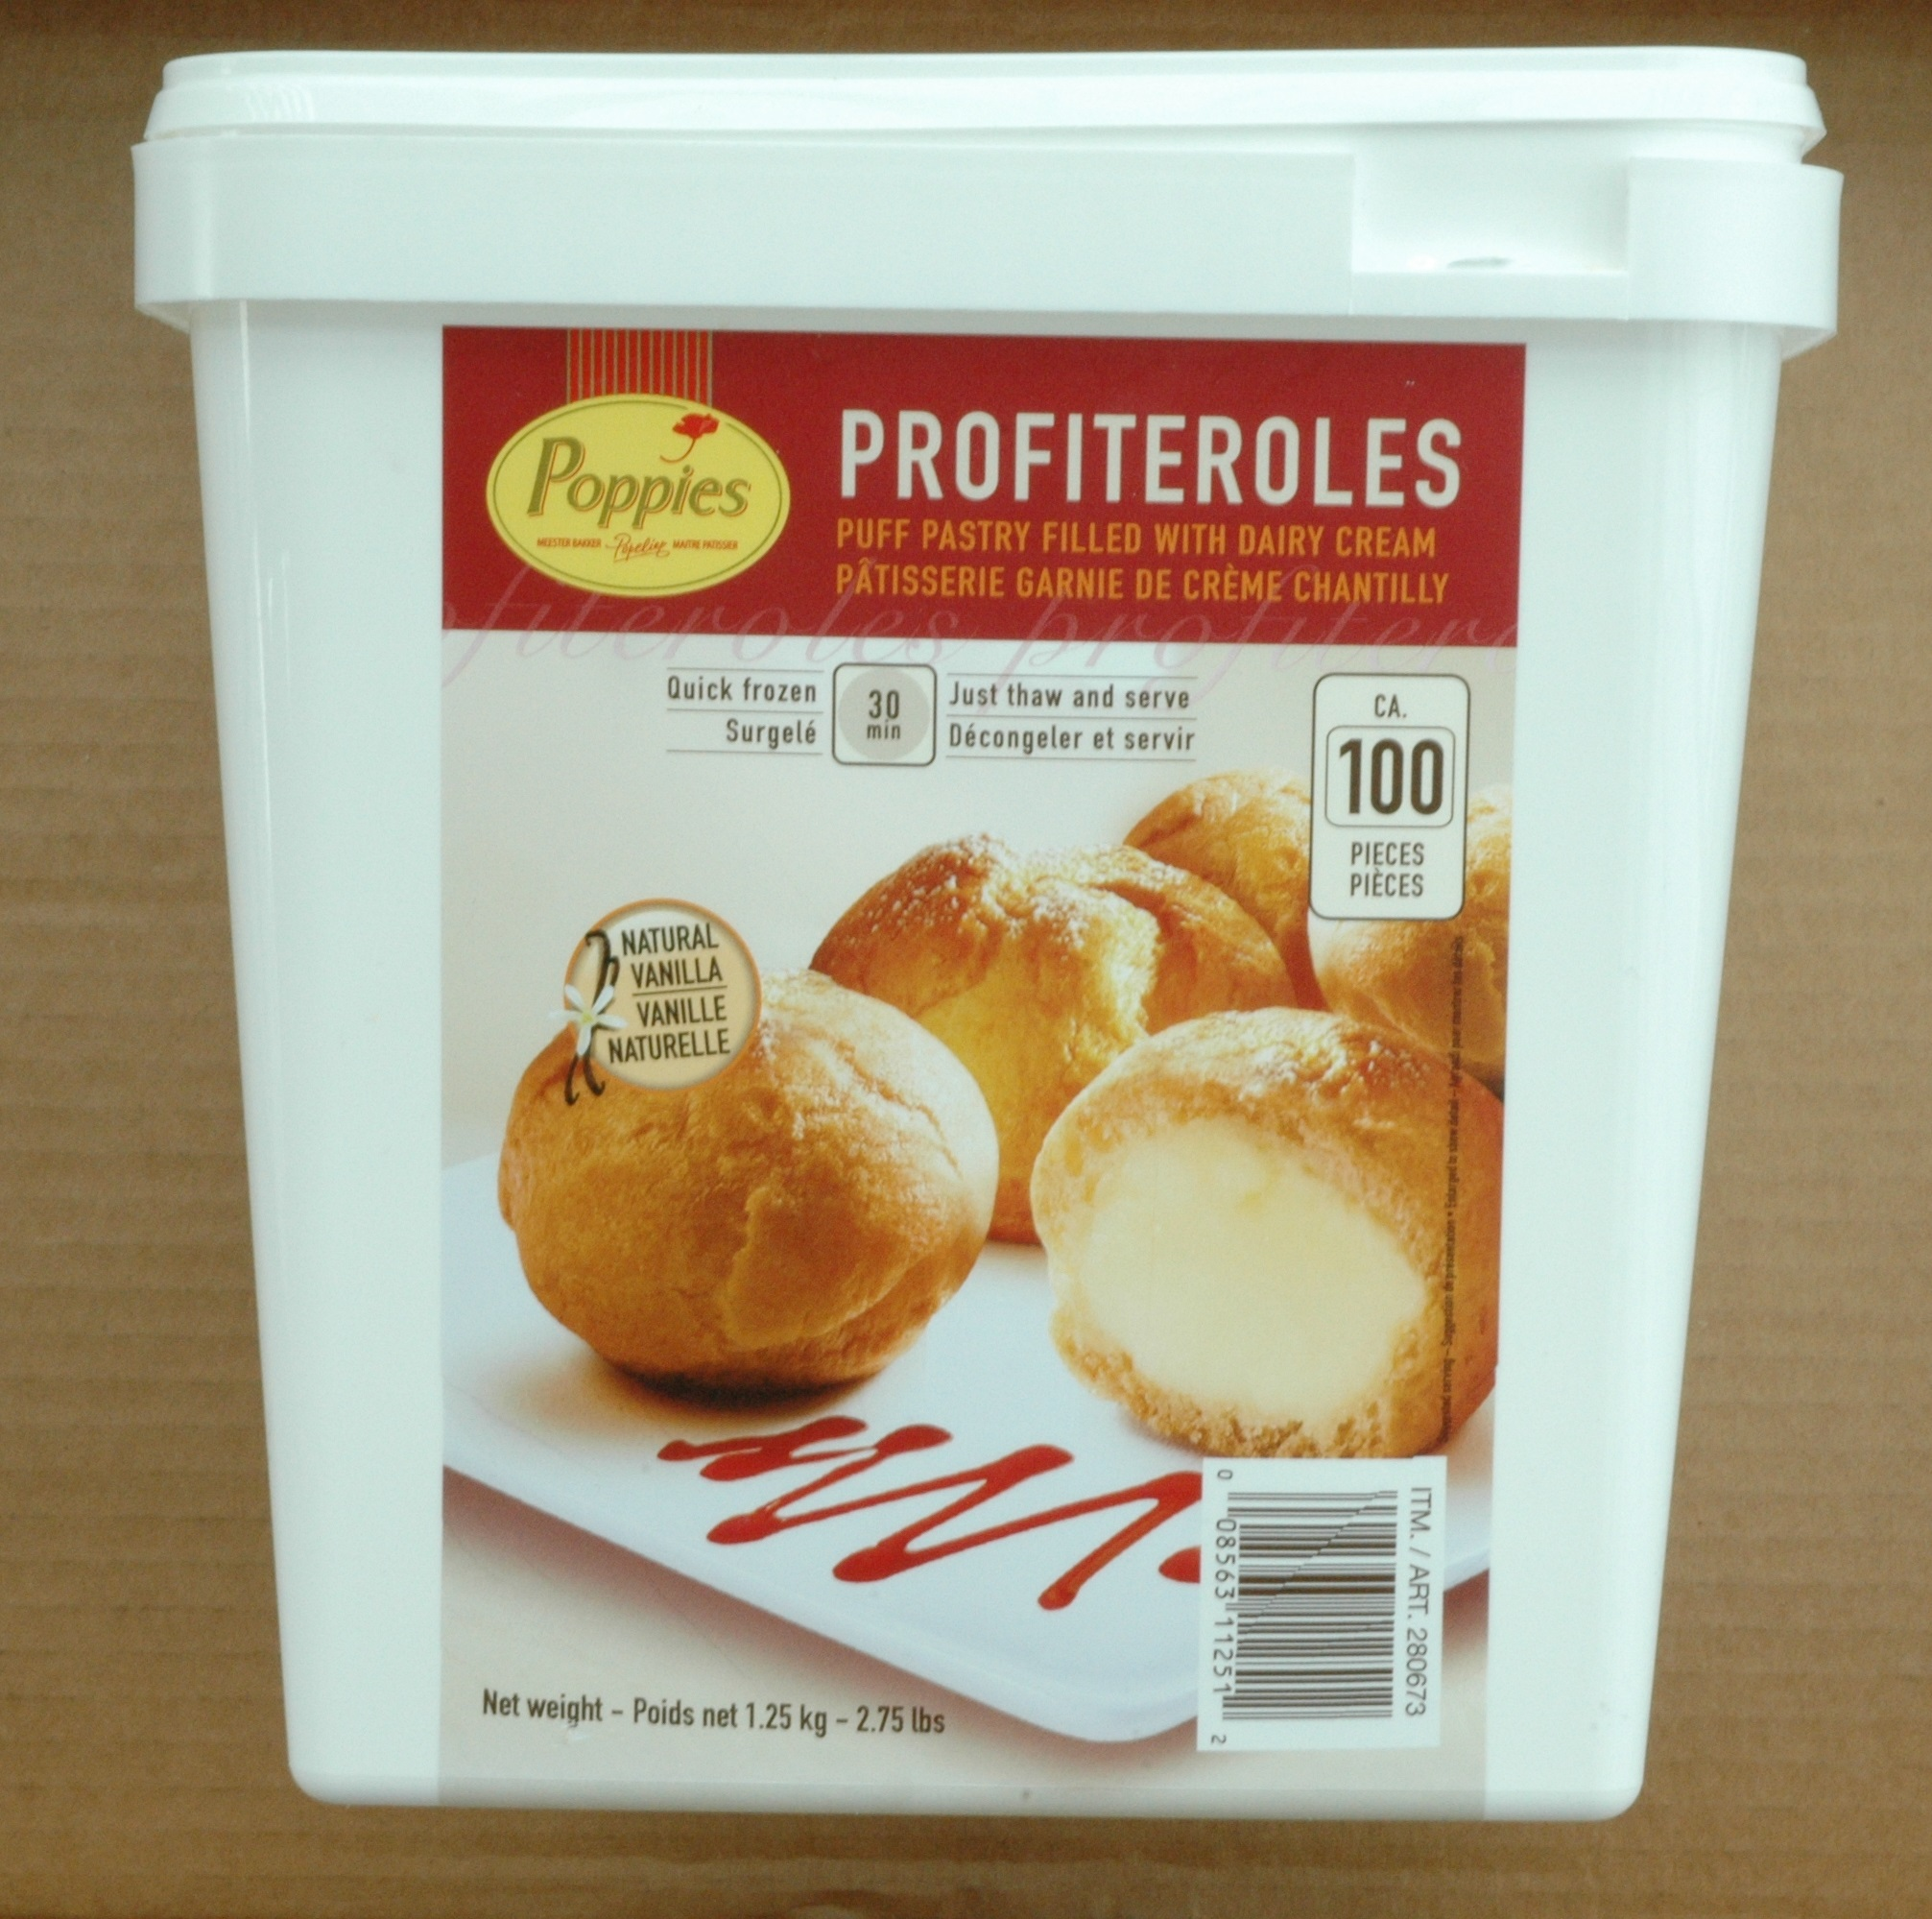
\includegraphics[width=0.33\textwidth]{interp/real_world_obj/box/box}} &
  \multicolumn{3}{l}{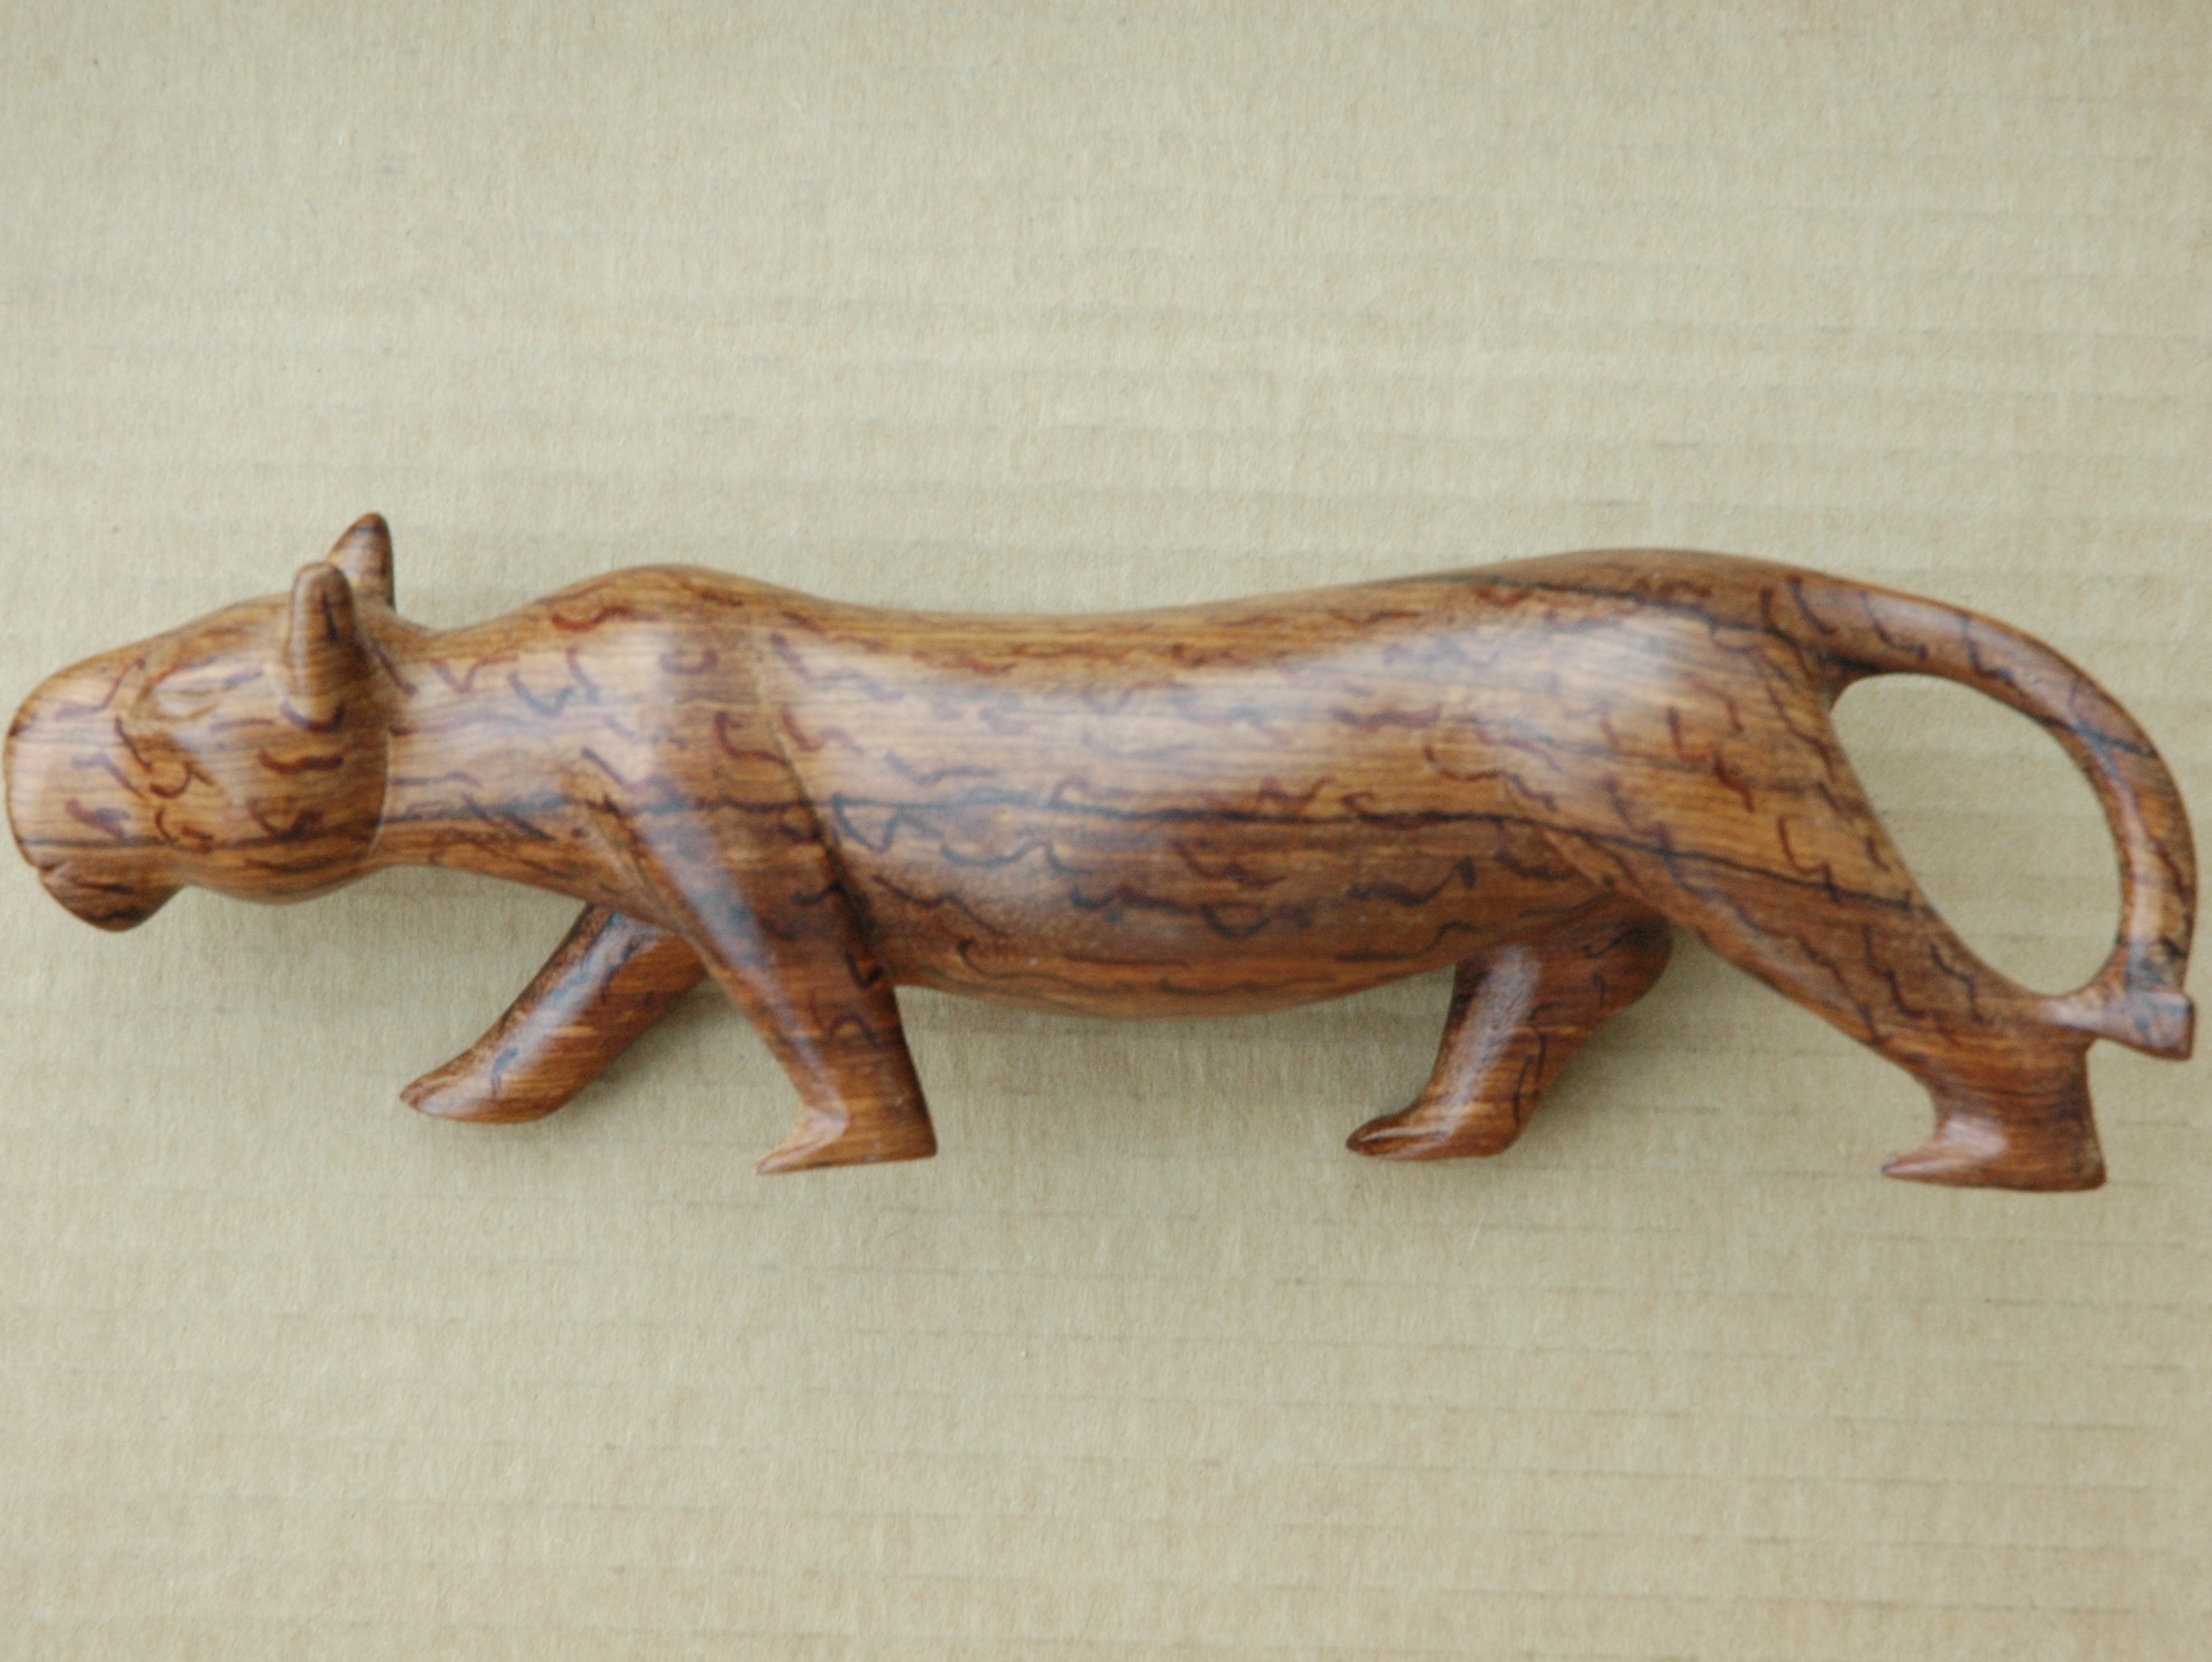
\includegraphics[width=0.33\textwidth]{interp/real_world_obj/cat0/cat0}} &
  \multicolumn{3}{l}{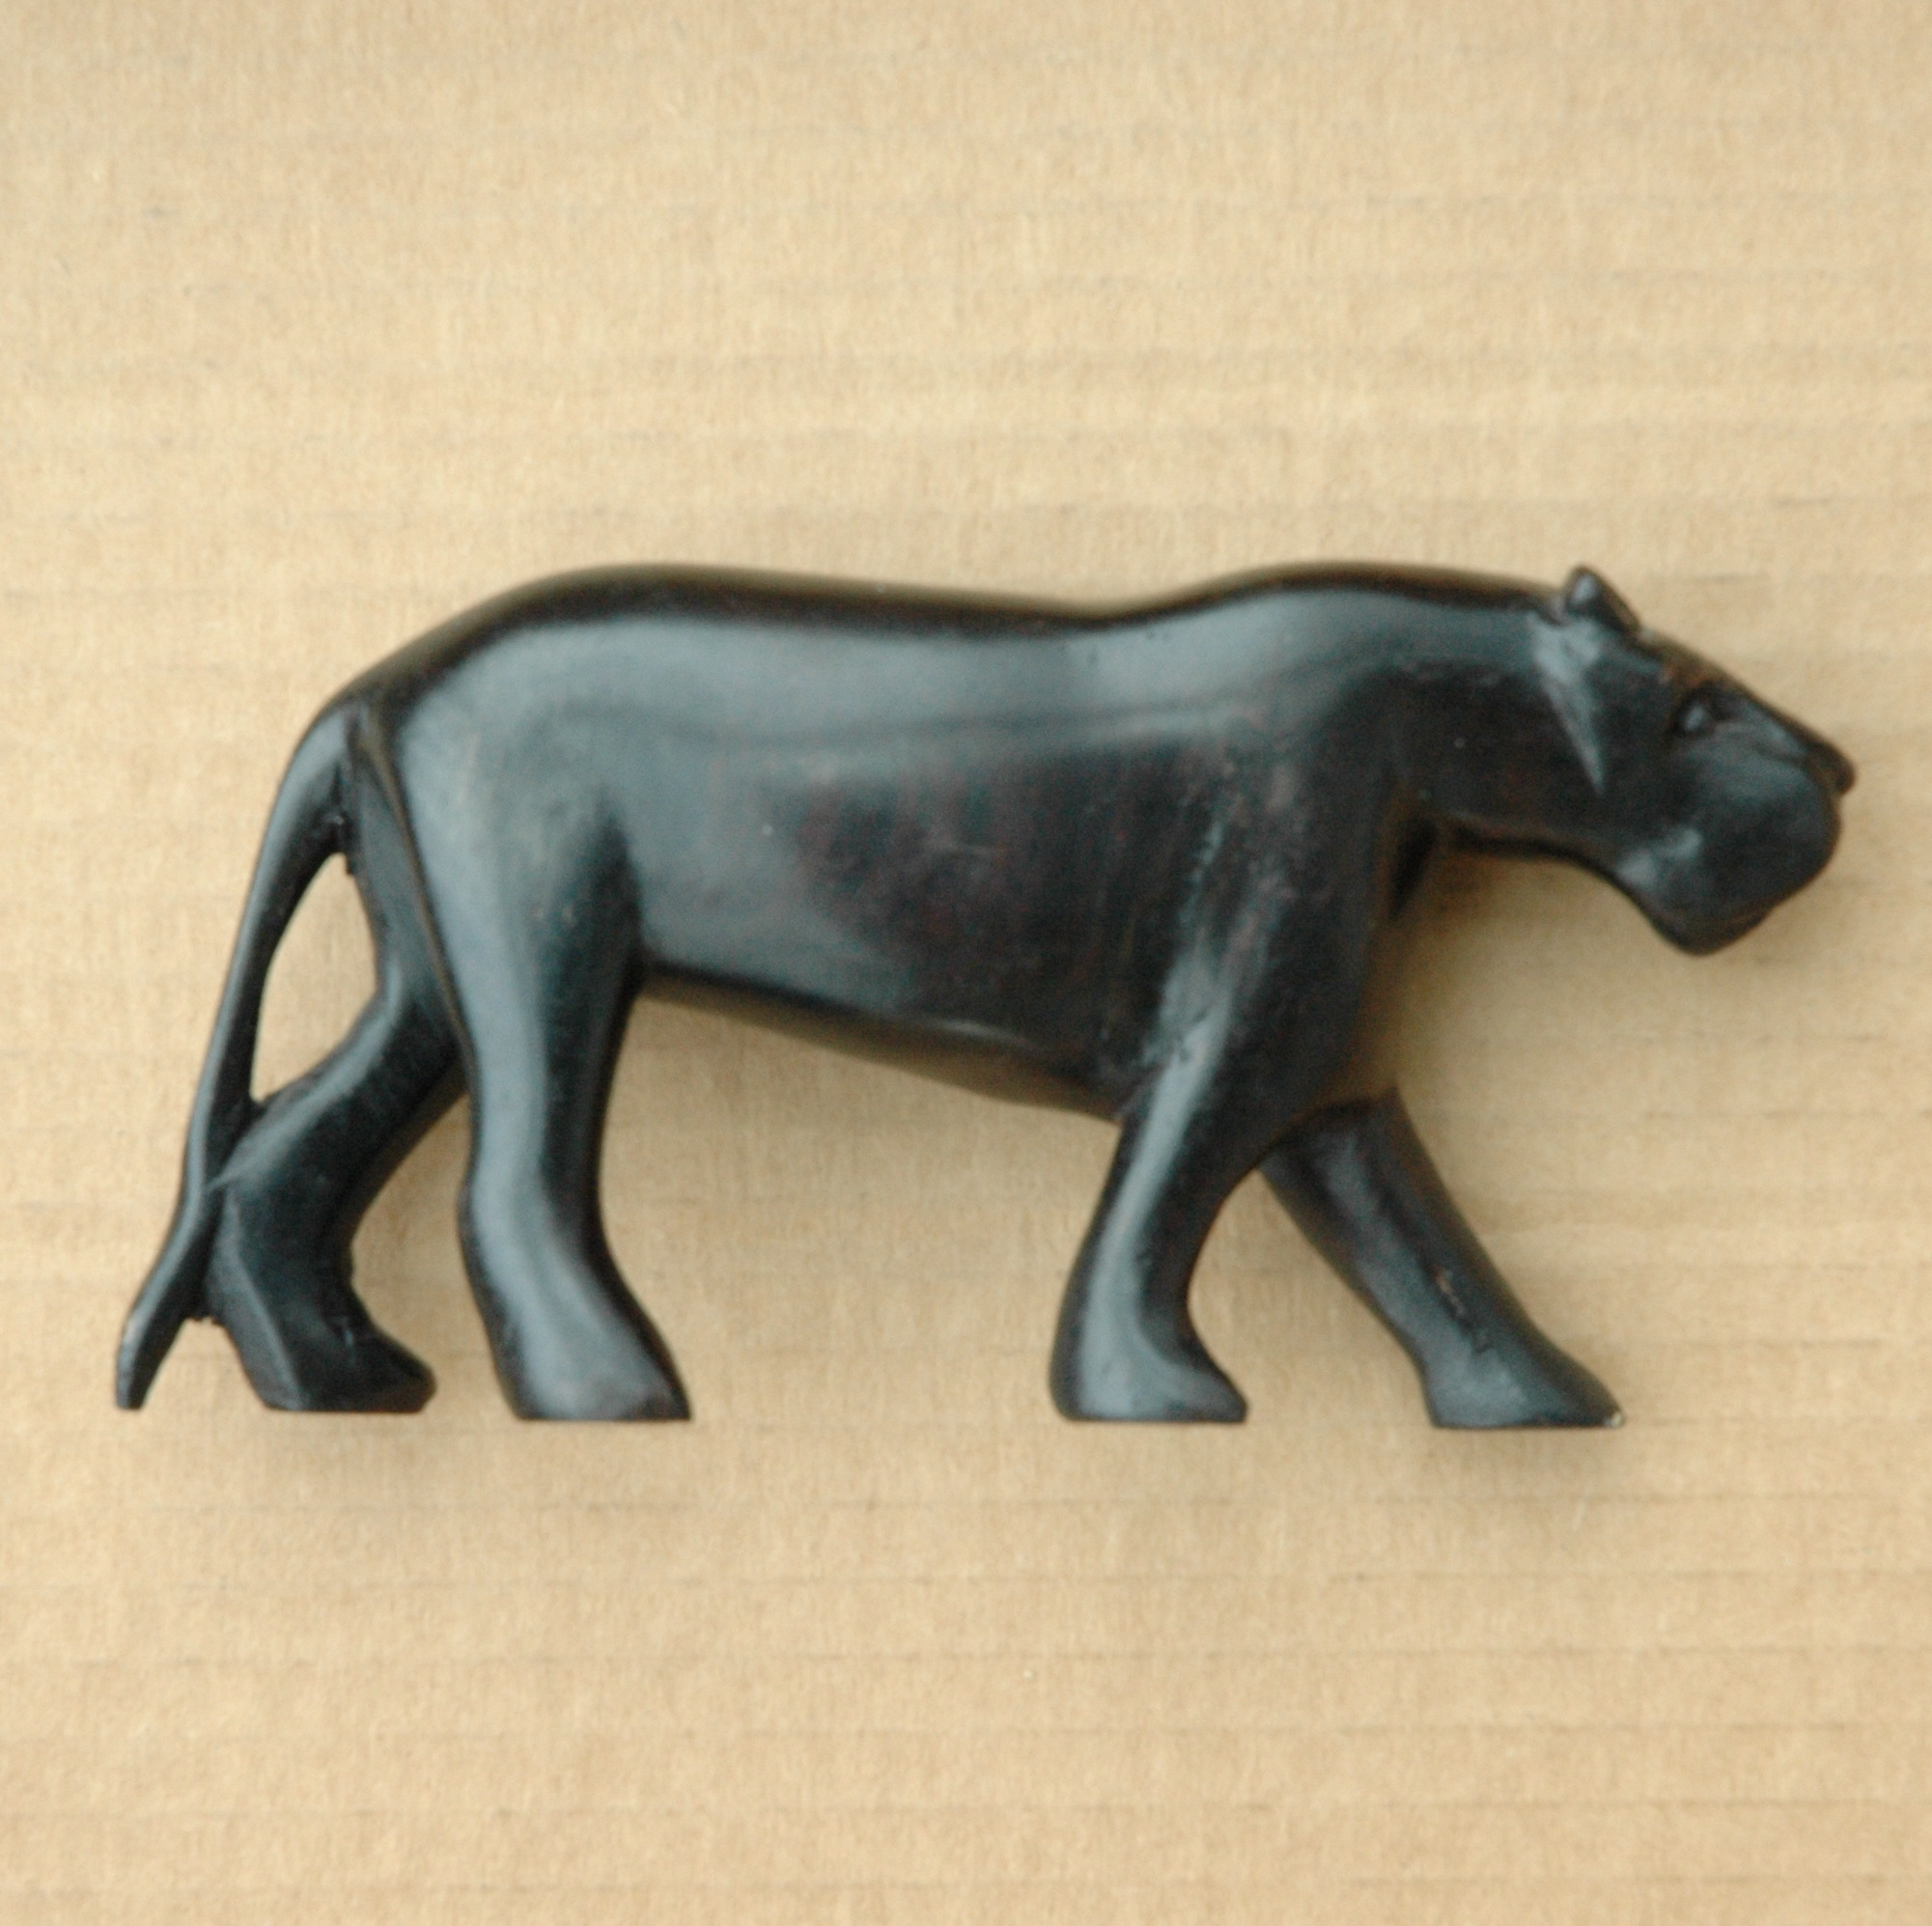
\includegraphics[width=0.33\textwidth]{interp/real_world_obj/cat1/cat1}}\\
  \includegraphics[width=0.1\textwidth]{interp/real_world_obj/box/base_00} &
  \includegraphics[width=0.1\textwidth]{interp/real_world_obj/box/base_01} & 
  \includegraphics[width=0.1\textwidth]{interp/real_world_obj/box/base_02} &
  \includegraphics[width=0.1\textwidth]{interp/real_world_obj/cat0/base_00} & 
  \includegraphics[width=0.1\textwidth]{interp/real_world_obj/cat0/base_01}& &
  \includegraphics[width=0.1\textwidth]{interp/real_world_obj/cat1/base_00} &\\
  \multicolumn{3}{c}{(a). box} & \multicolumn{3}{c}{(b). cat0} & \multicolumn{3}{c}{(c). cat1} \\
  \multicolumn{3}{l}{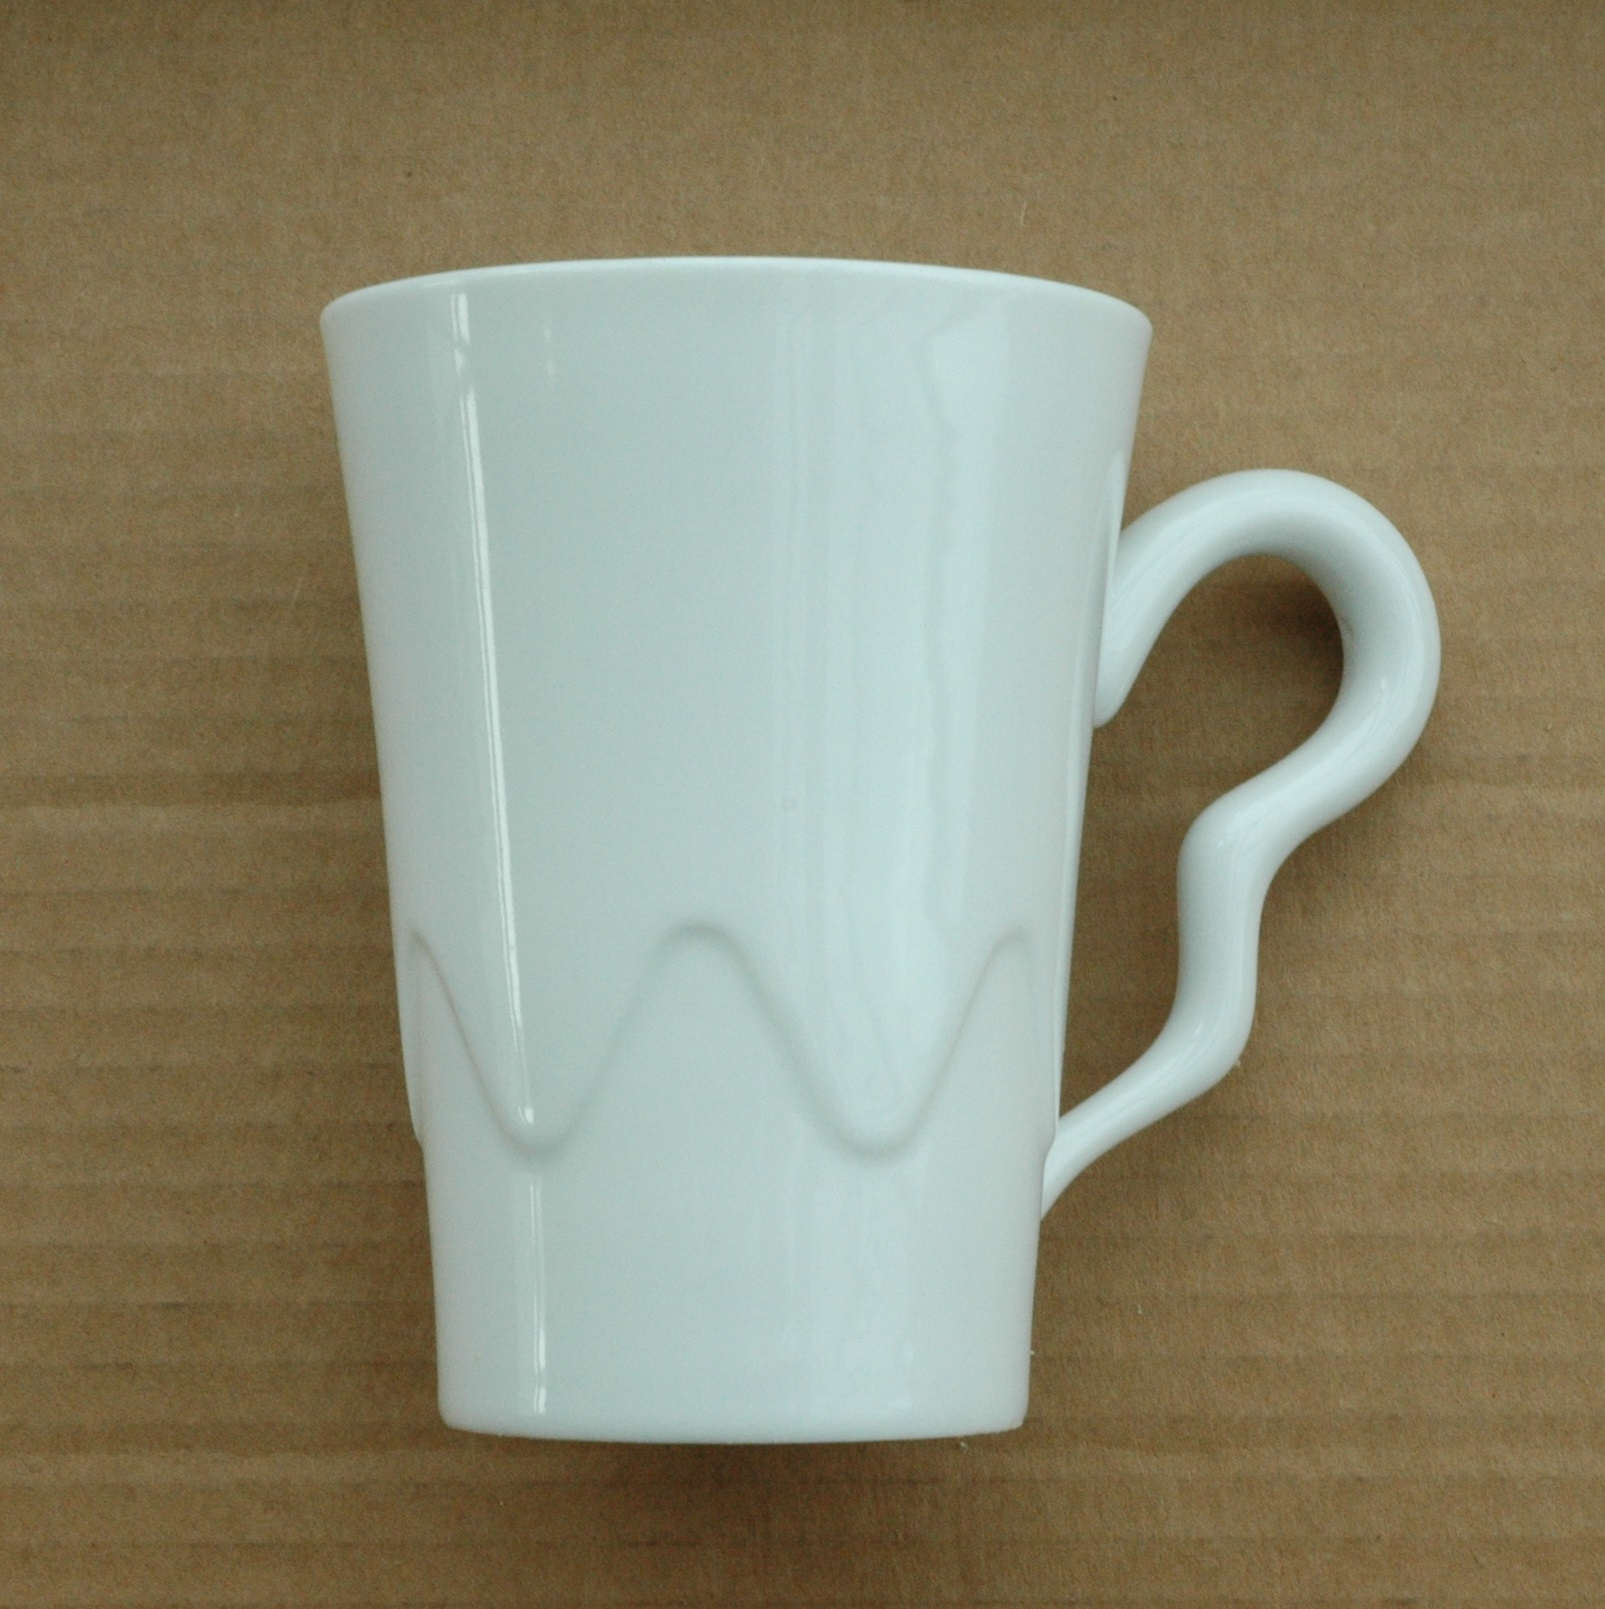
\includegraphics[width=0.33\textwidth]{interp/real_world_obj/cup/cup}} &
  \multicolumn{3}{l}{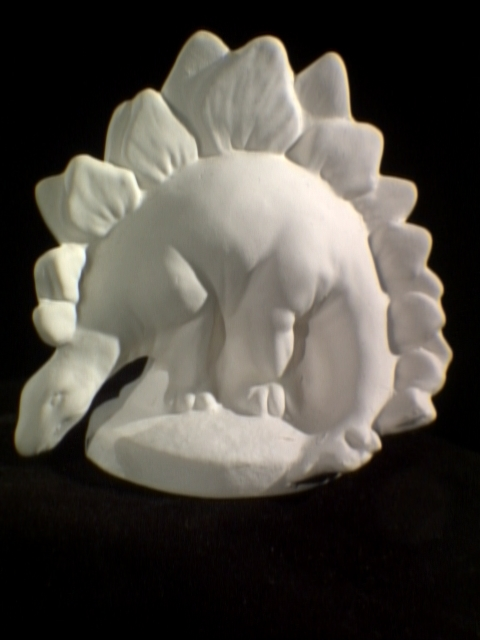
\includegraphics[width=0.33\textwidth]{interp/real_world_obj/dino/dino}} &
  \multicolumn{3}{l}{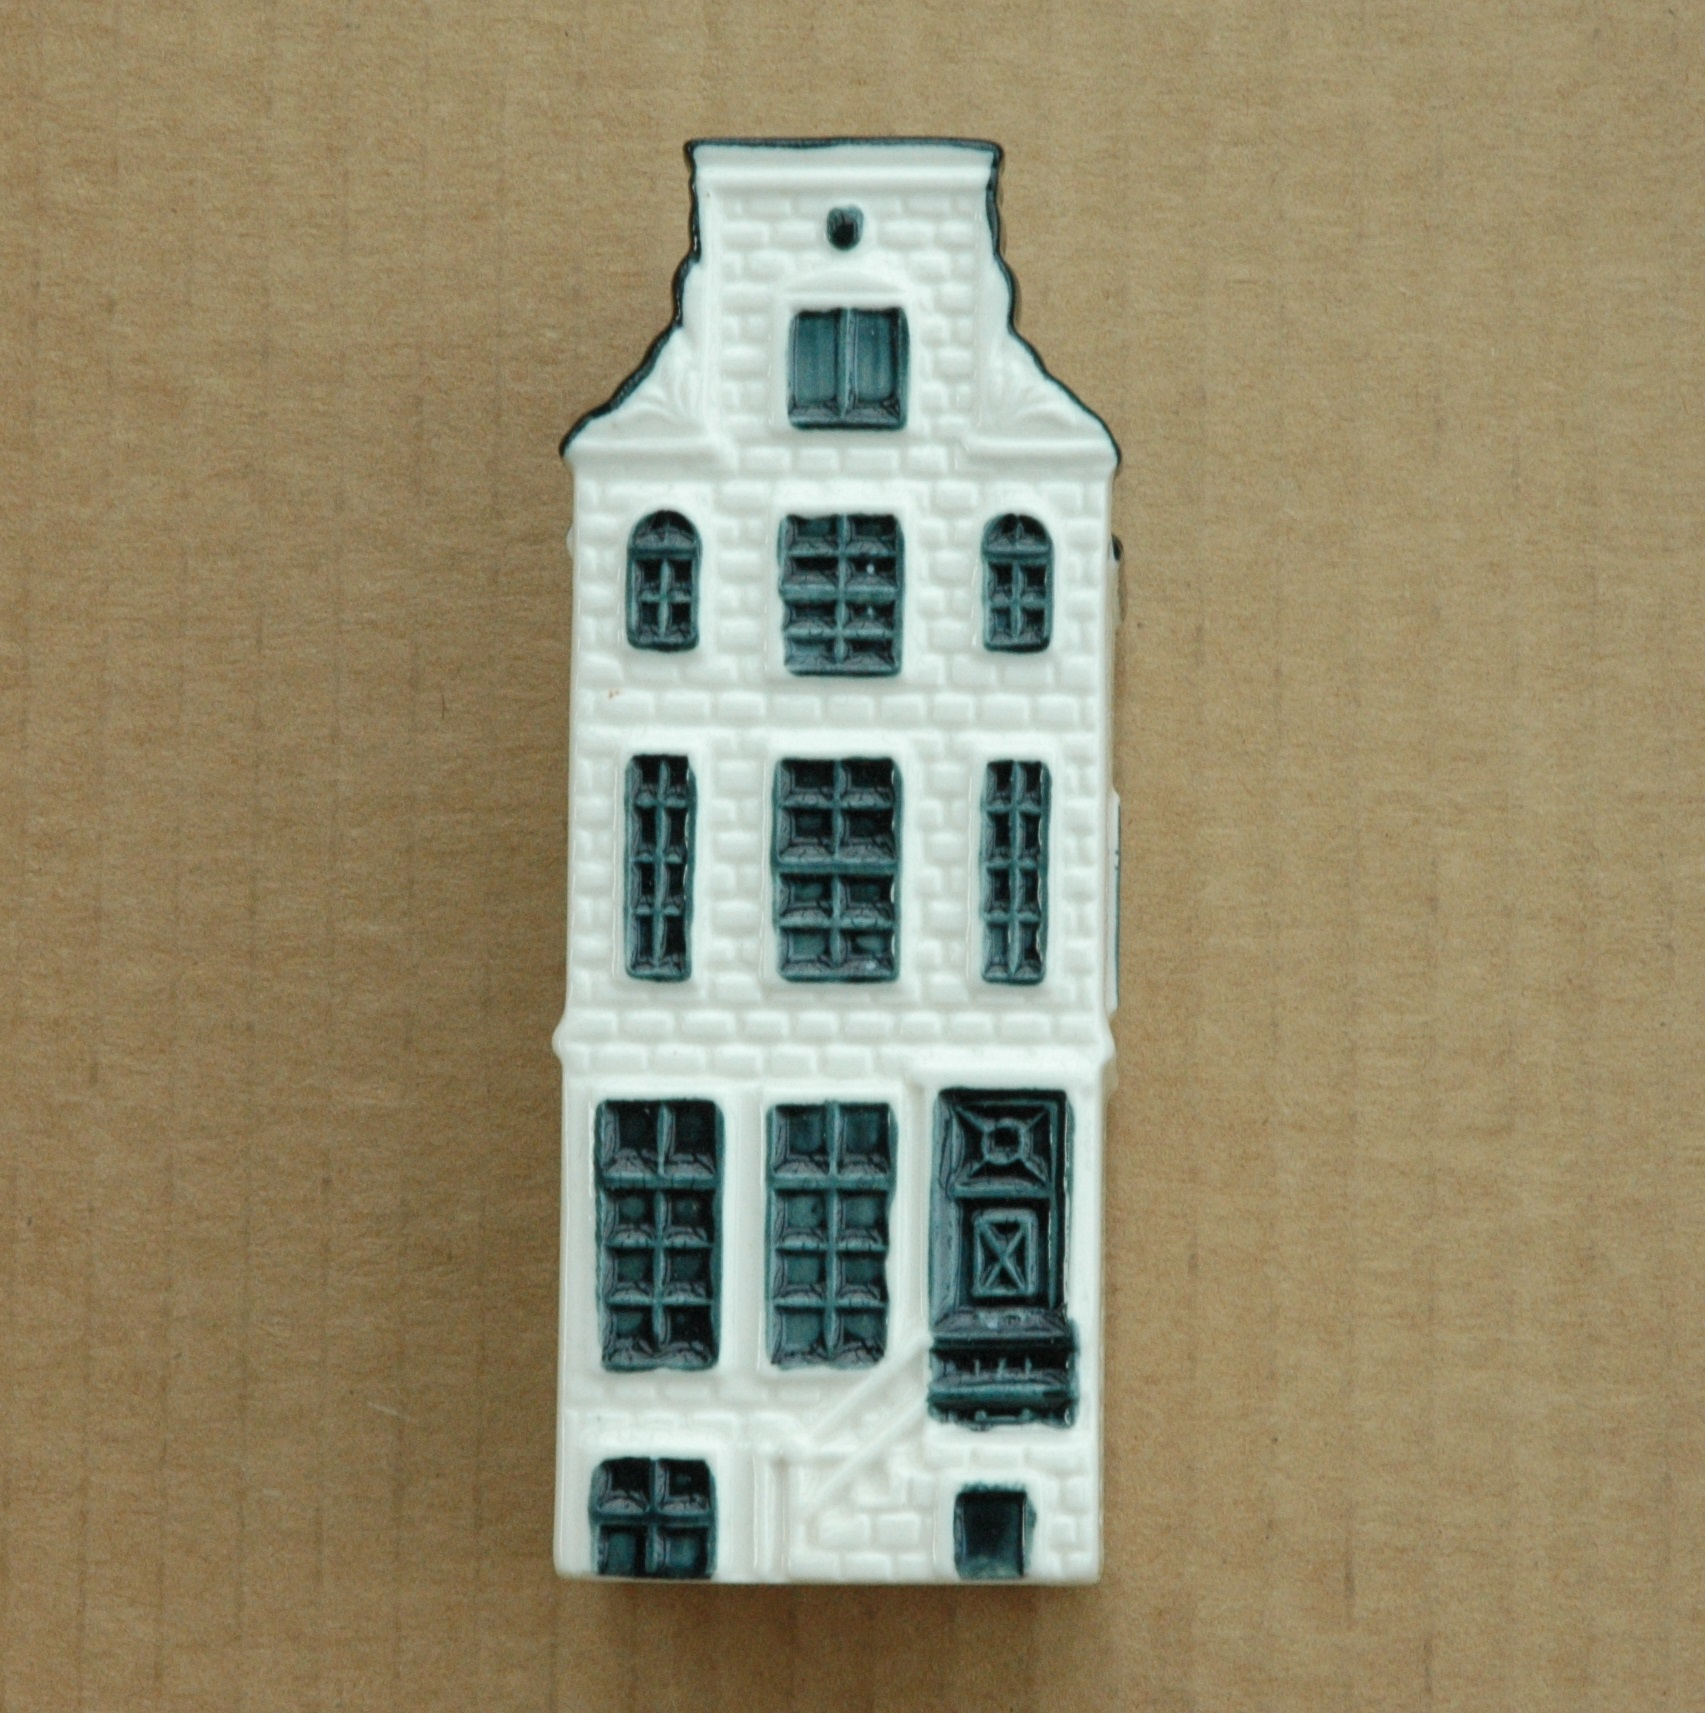
\includegraphics[width=0.33\textwidth]{interp/real_world_obj/house/house}}\\
  \includegraphics[width=0.1\textwidth]{interp/real_world_obj/cup/base_00} & & &
  \includegraphics[width=0.1\textwidth]{interp/real_world_obj/dino/base_00} & 
  \includegraphics[width=0.1\textwidth]{interp/real_world_obj/dino/base_01} & 
  \includegraphics[width=0.1\textwidth]{interp/real_world_obj/dino/base_02} &
  \includegraphics[width=0.1\textwidth]{interp/real_world_obj/house/base_00} &
  \includegraphics[width=0.1\textwidth]{interp/real_world_obj/house/base_01} & \\
  \multicolumn{3}{c}{(d). cup} & \multicolumn{3}{c}{(e). dino} & \multicolumn{3}{c}{(f). house} \\
  \multicolumn{3}{l}{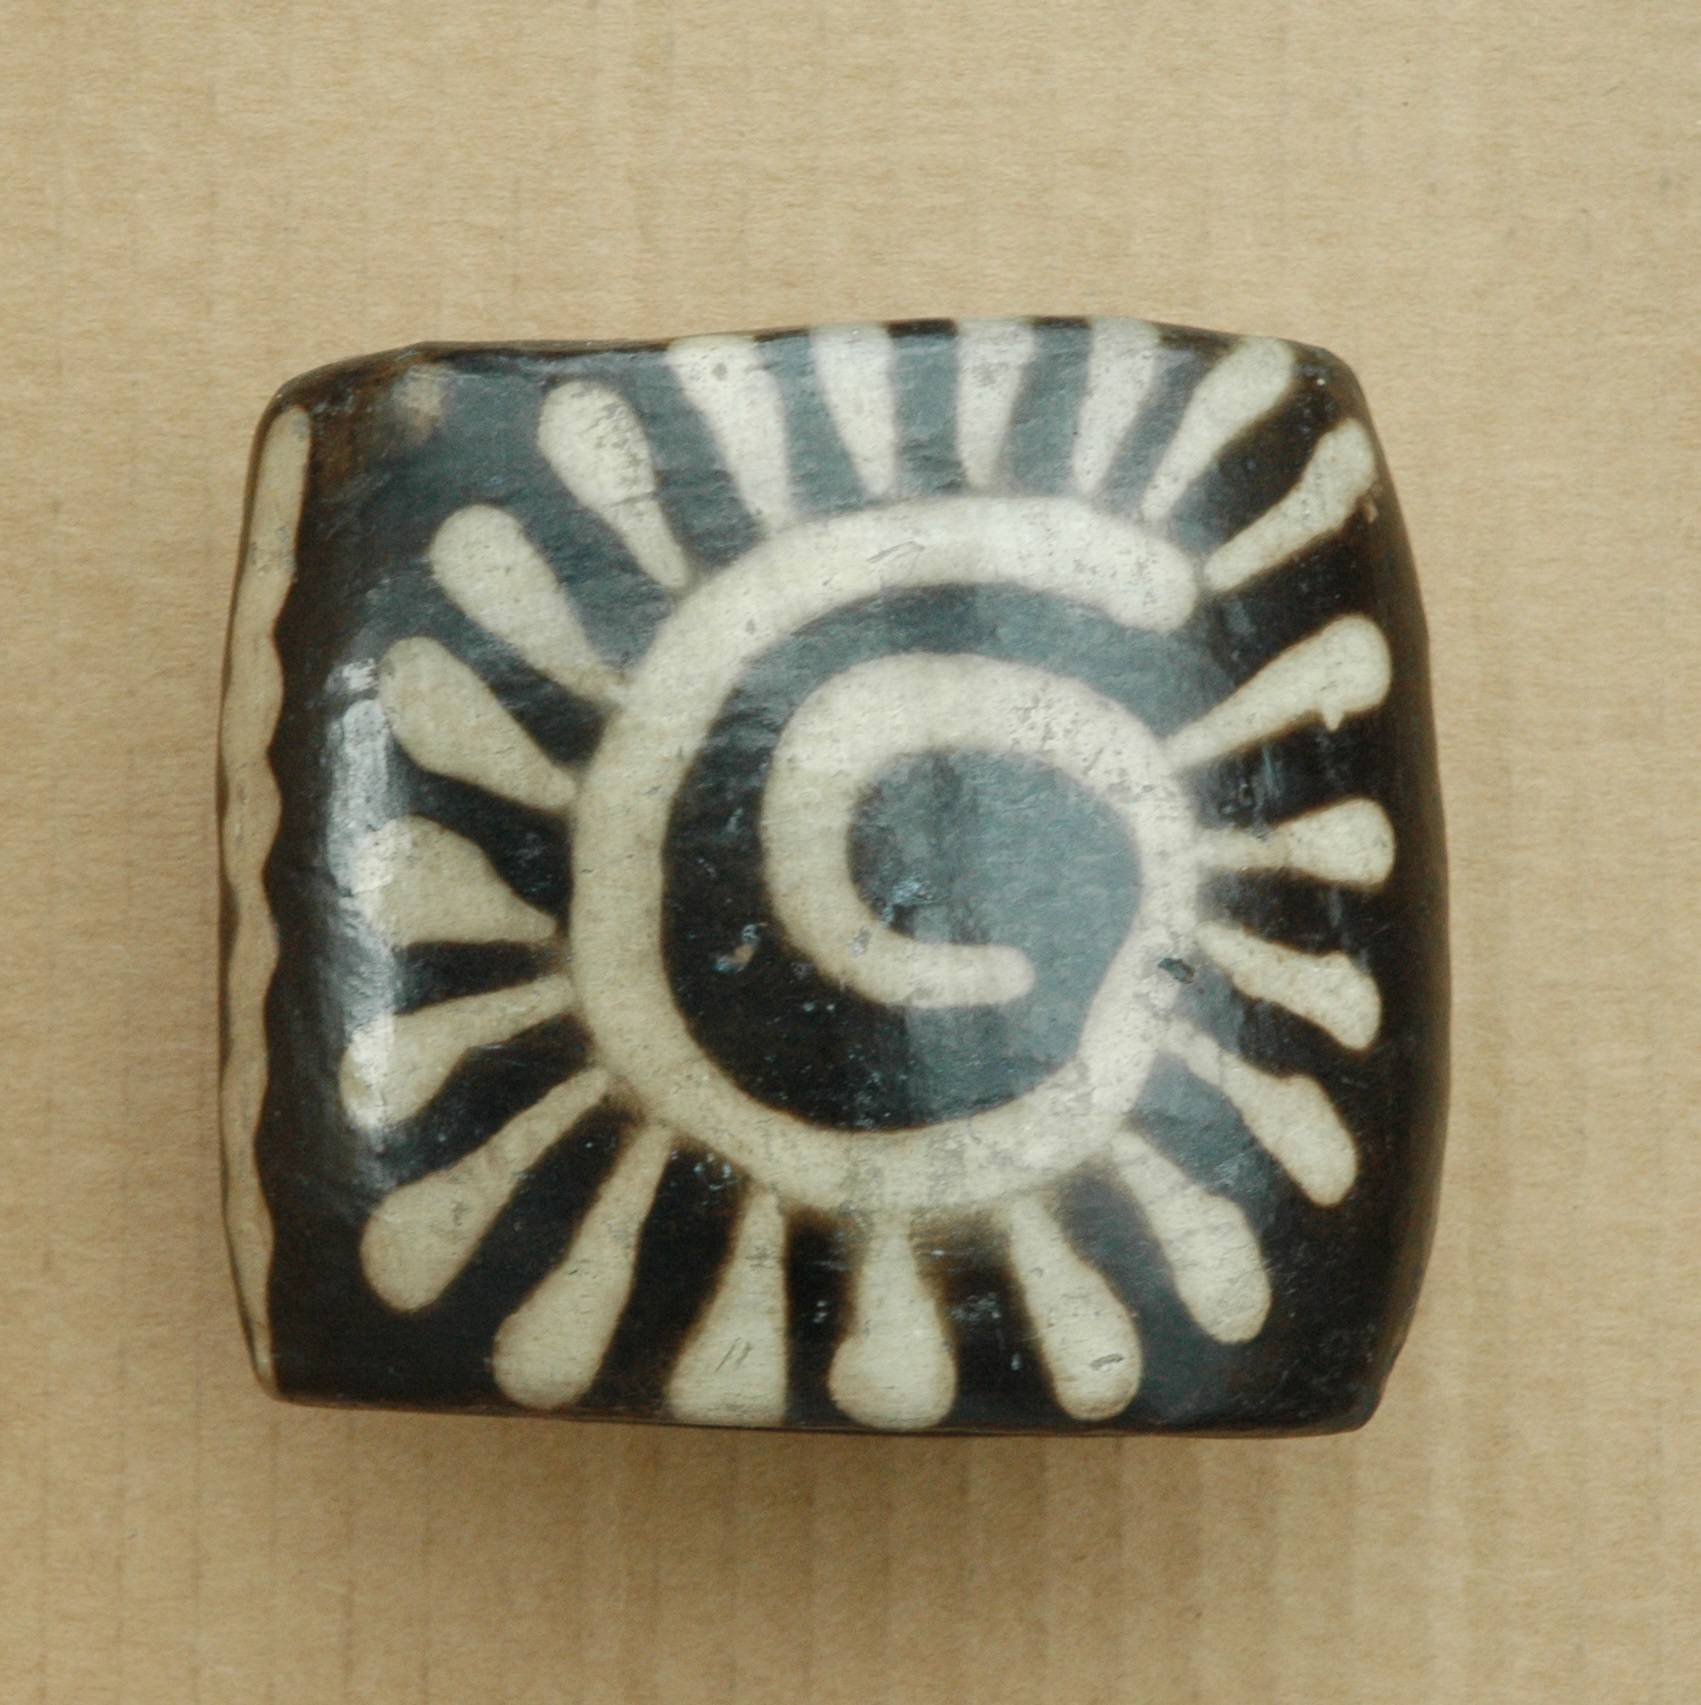
\includegraphics[width=0.33\textwidth]{interp/real_world_obj/pot/pot}} &
  \multicolumn{3}{l}{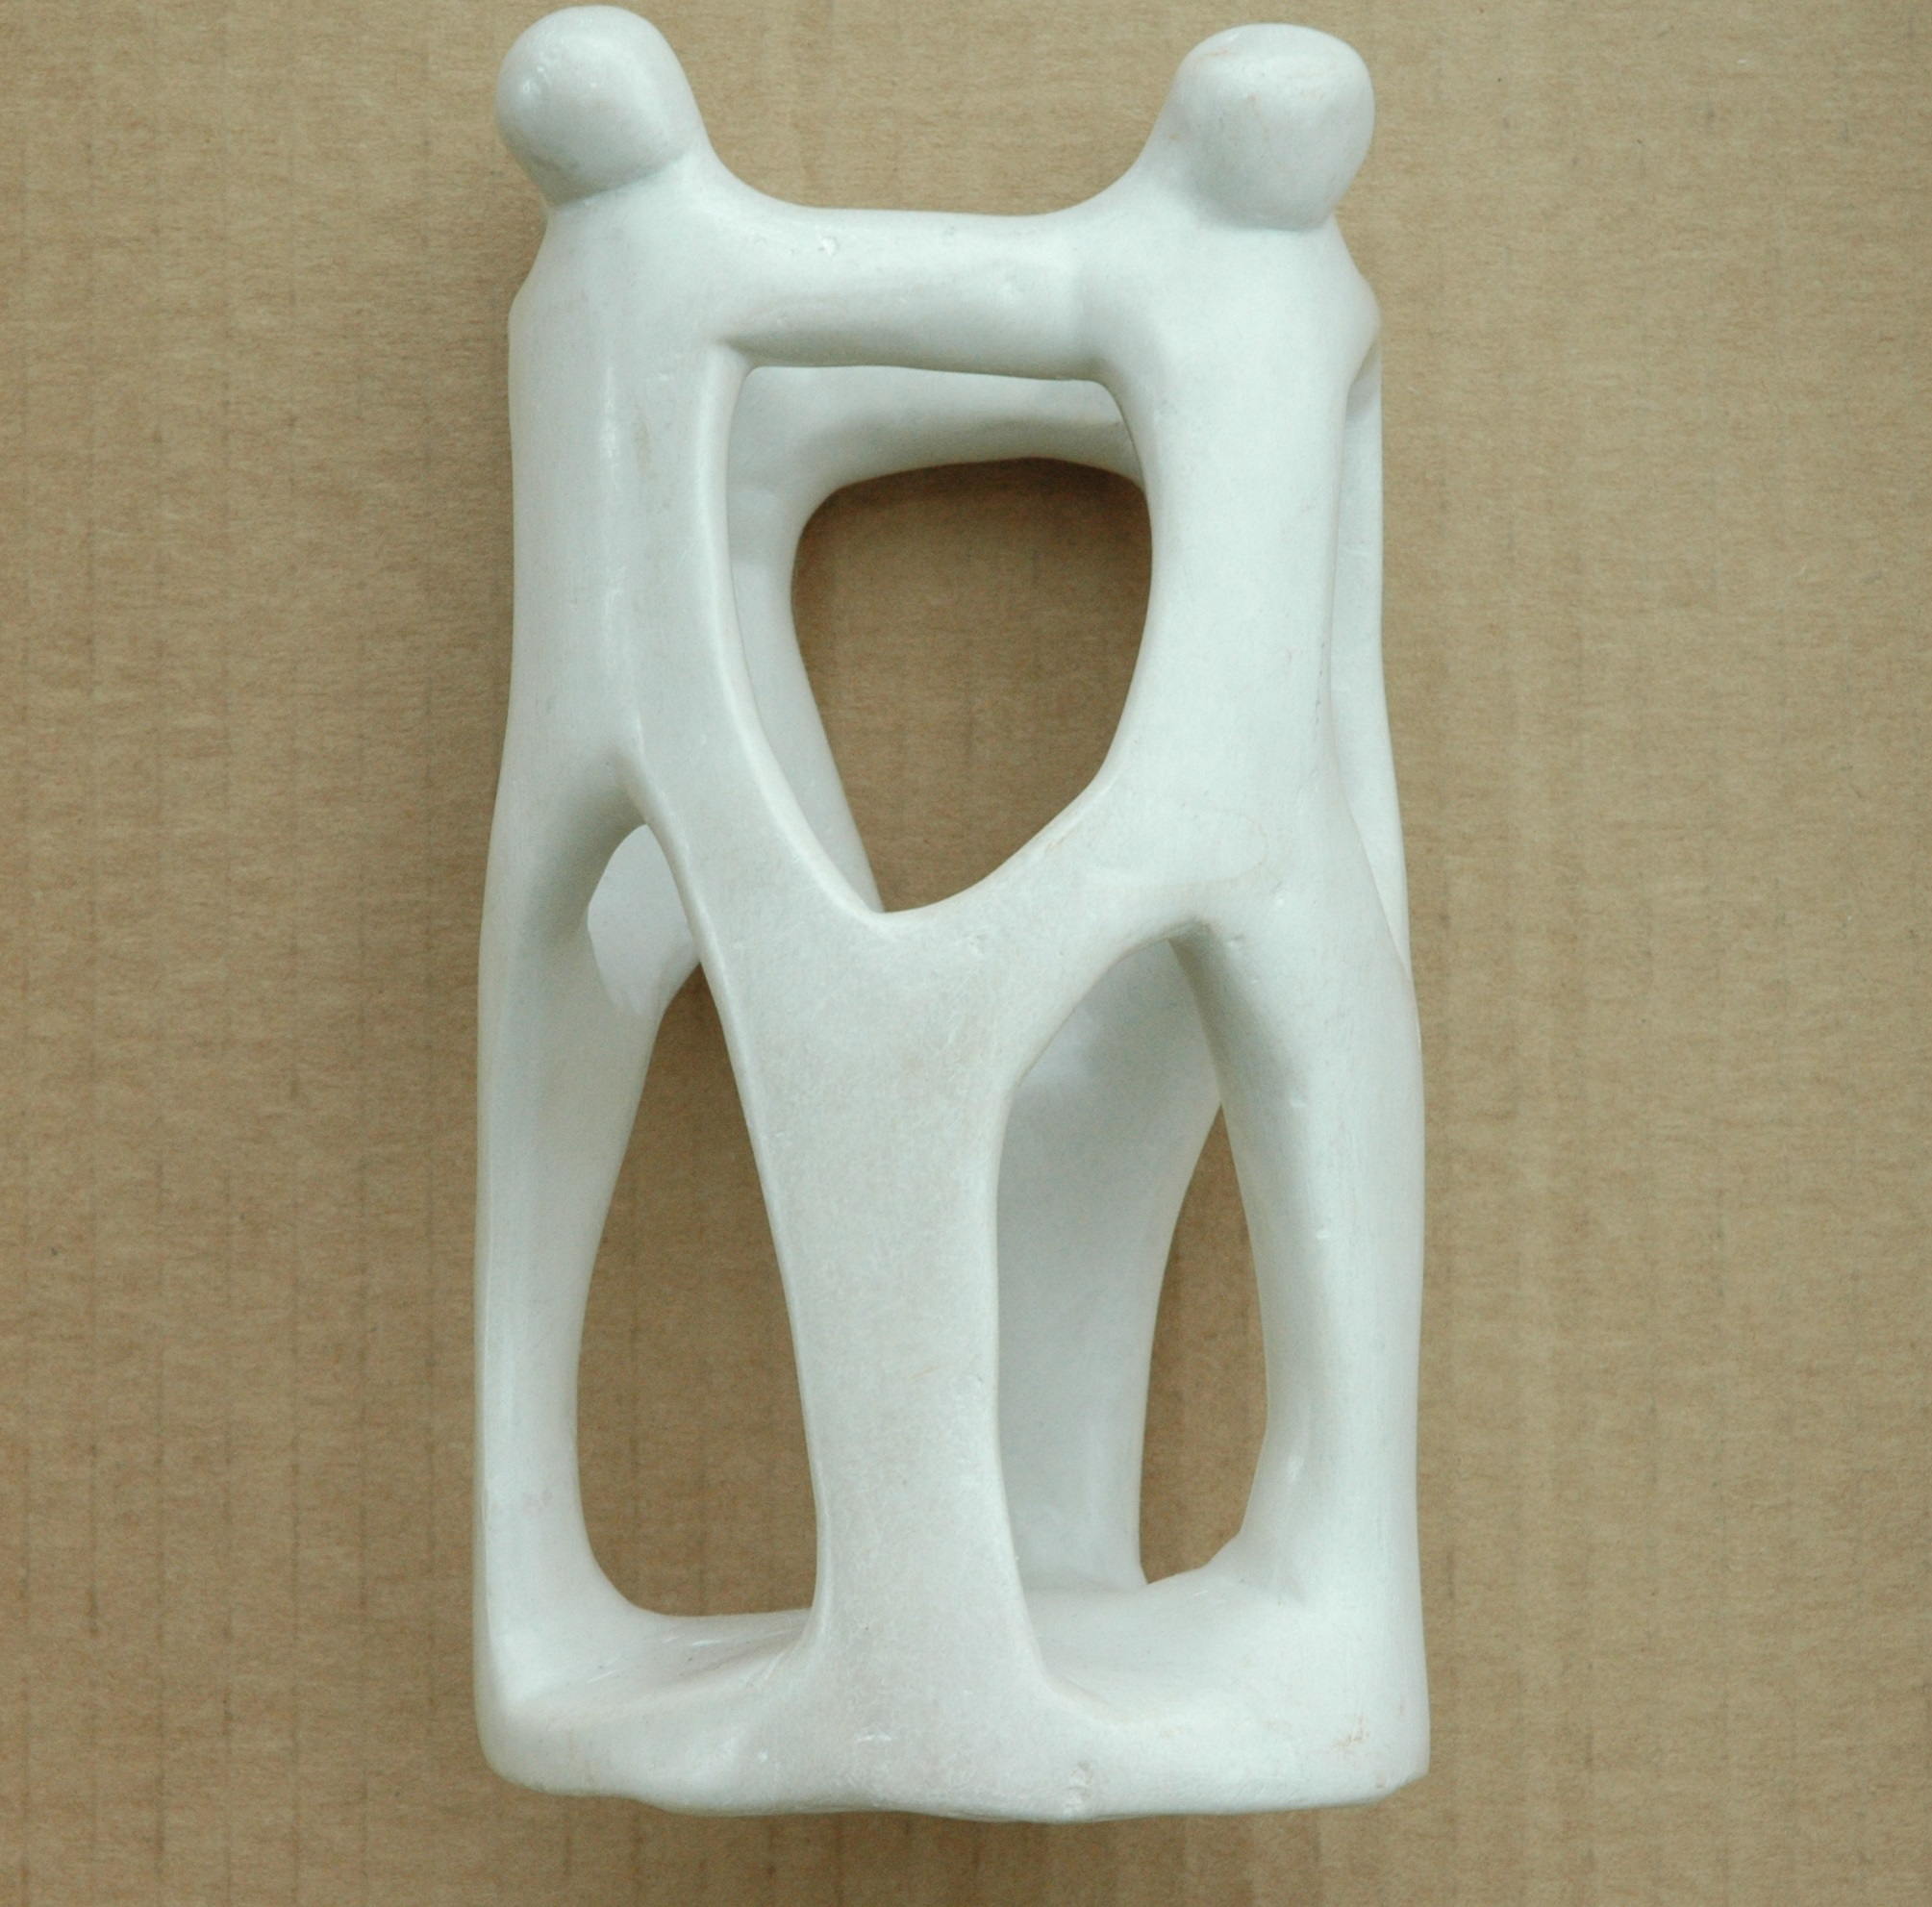
\includegraphics[width=0.33\textwidth]{interp/real_world_obj/statue/statue}} &
  \multicolumn{3}{l}{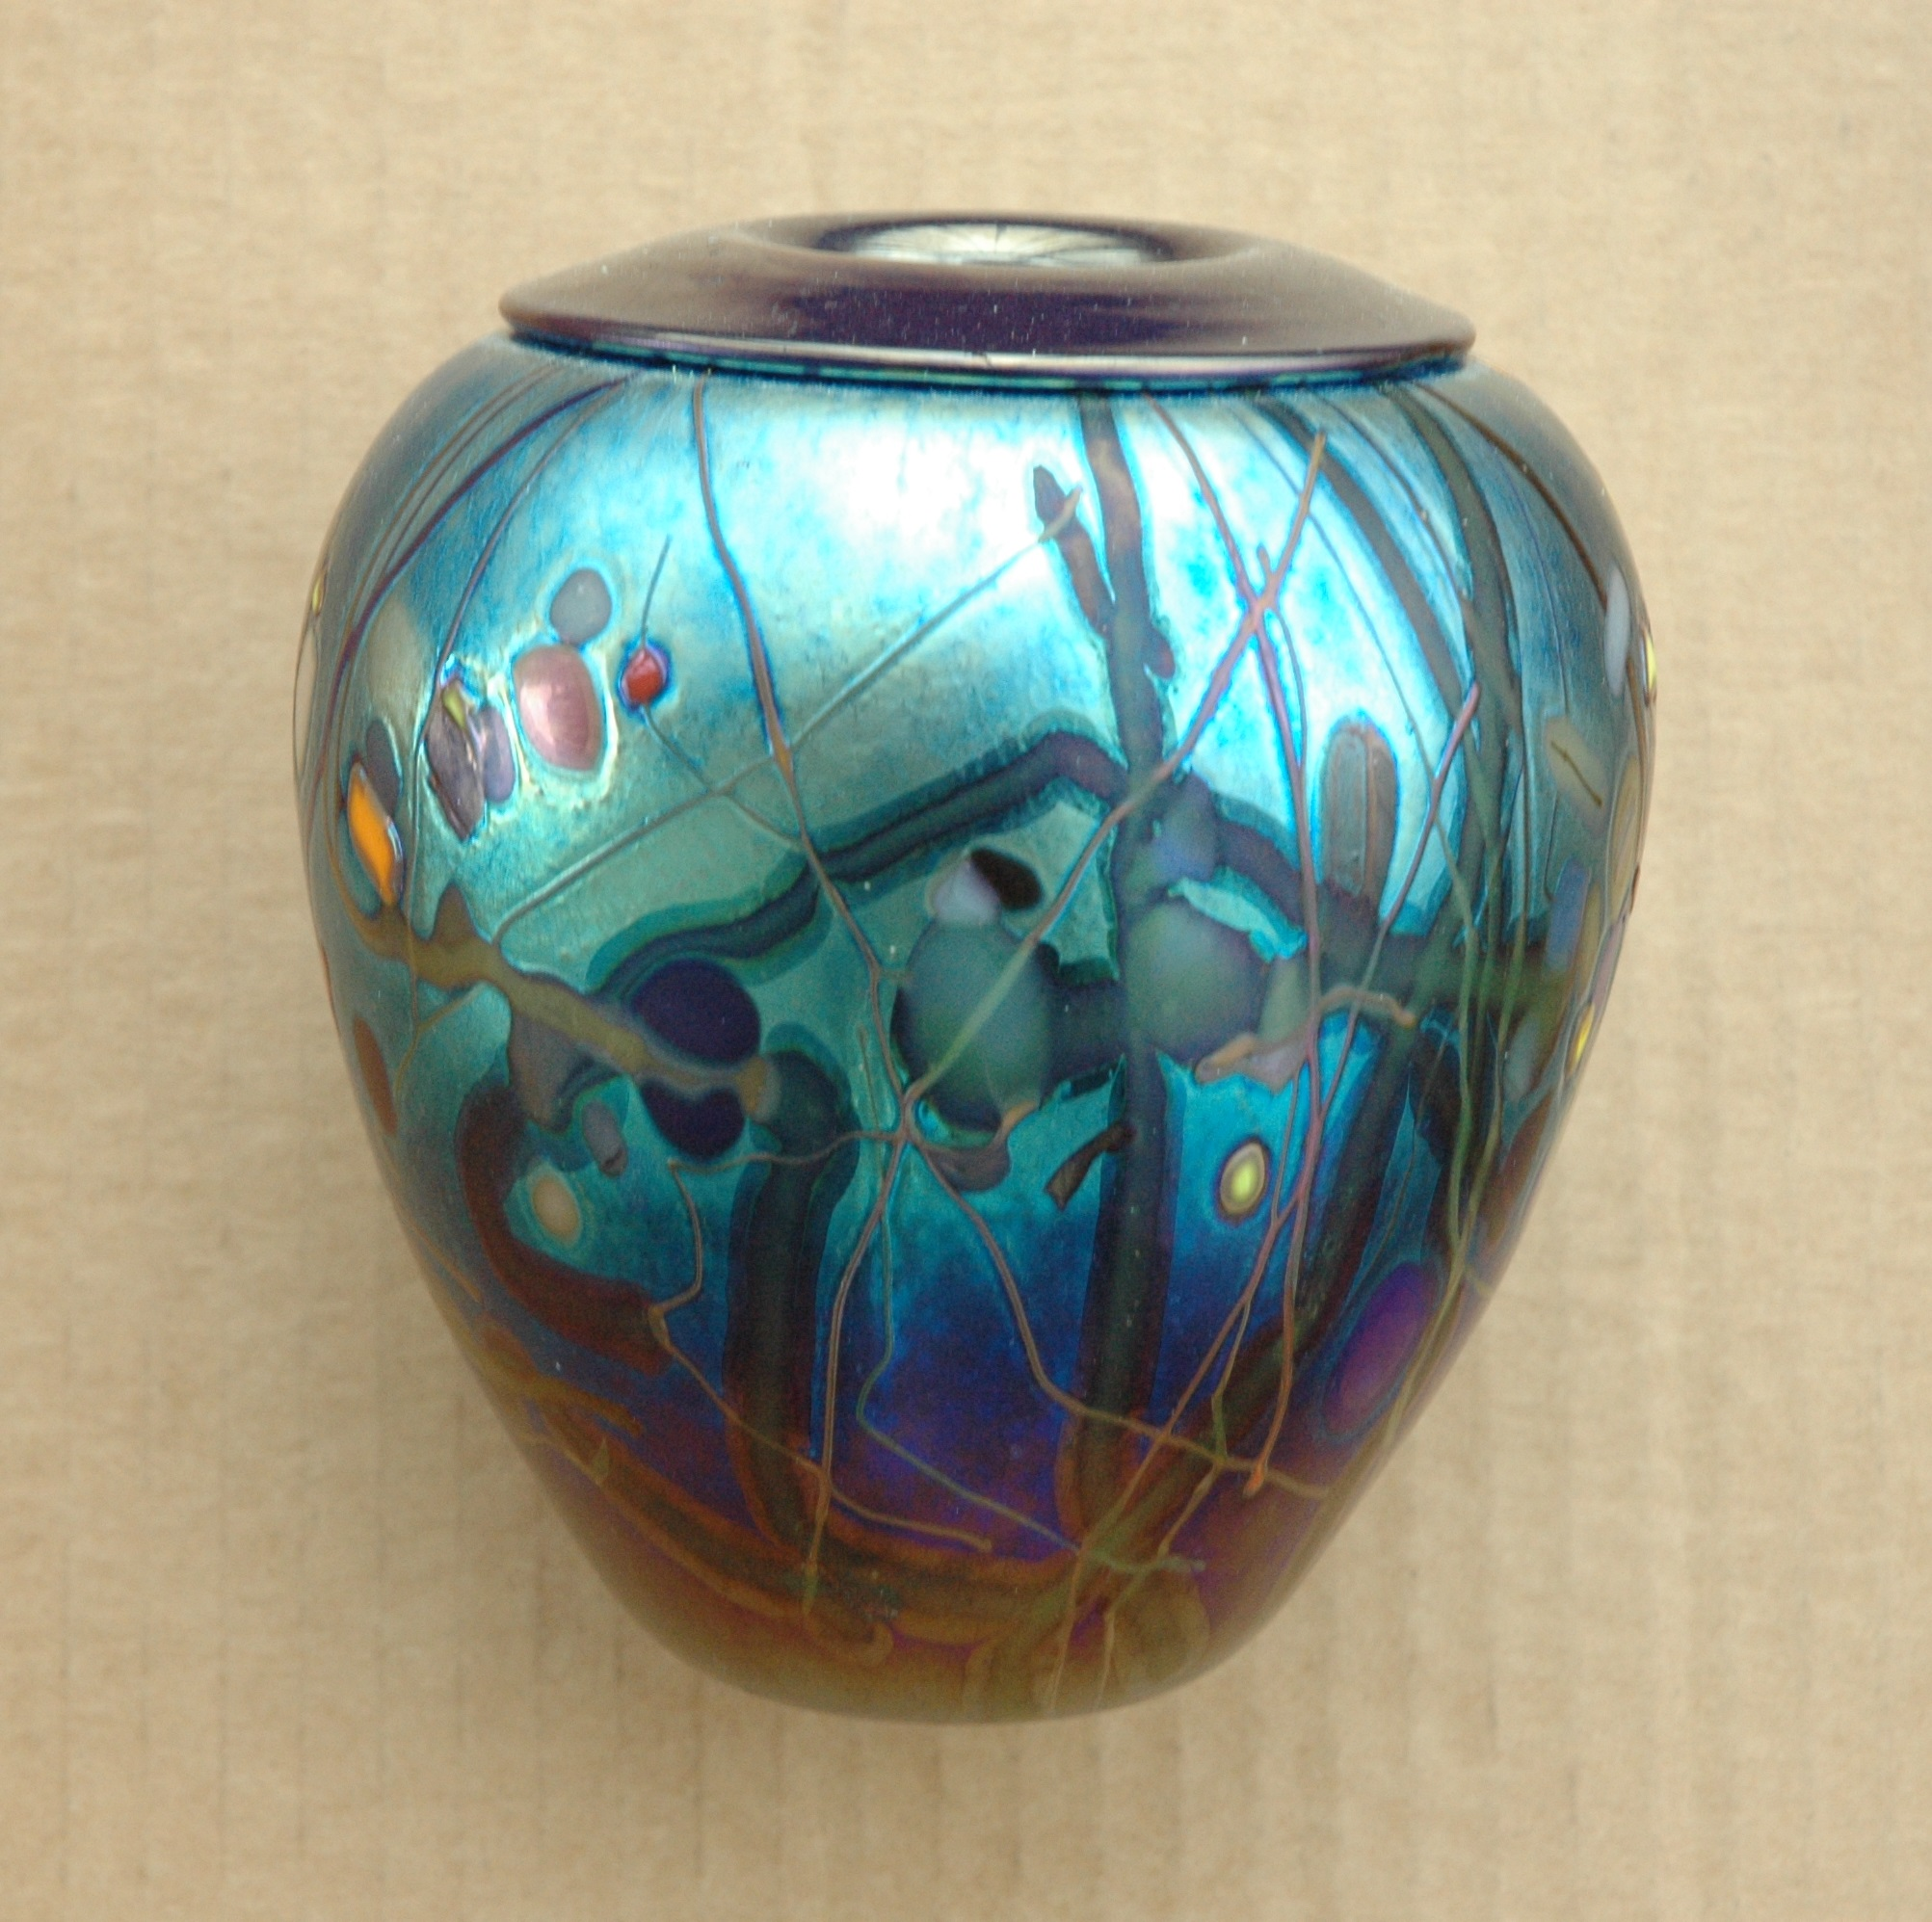
\includegraphics[width=0.33\textwidth]{interp/real_world_obj/vase/vase}}\\
  \includegraphics[width=0.1\textwidth]{interp/real_world_obj/pot/base_00} &
  \includegraphics[width=0.1\textwidth]{interp/real_world_obj/pot/base_01} & &
  \includegraphics[width=0.1\textwidth]{interp/real_world_obj/statue/base_00} & & &
  \includegraphics[width=0.1\textwidth]{interp/real_world_obj/vase/base_00} &
  \includegraphics[width=0.1\textwidth]{interp/real_world_obj/vase/base_01}\\
  \multicolumn{3}{c}{(g). pot} & \multicolumn{3}{c}{(h). statue} & \multicolumn{3}{c}{(i). vase} \\
  \end{tabular}
  \caption{Material of Real-world objects.}
  \label{fig:real_data_material}
\end{table}

\section{Parameters of real-world objects}
\begin{table}[!htbp]
  \centering
  \begin{tabular}{l*{5}{c}}
  \hline
  \textbf{Property} & Texture & Albedo & Specular & Roughness & Best-suited Algo.\\
  \hline
  box & 0.2 & 0.8 & 0.2 & 0.2 & MVS, SL, PS\\
      & 0.5 & 0.2 & 0.2 & 0.5 & \\
      & 0.8 & 0.8 & 0.2 & 0.5 & \\
  cat0 & 0.5 & 0.5, 0.2 & 0.2 & 0.2 & None\\
  cat1 & 0.2 & 0.2 & 0.2 & 0.2 & None\\
  cup & 0.2 & 0.8 & 0.2 & 0.2 & PS, SL\\
  dino & 0.2 & 0.5, 0.8, 0.8 & 0.2 & 0.5 & SL\\
  house & 0.8 & 0.8, 0.2 & 0.2 & 0.2 & MVS\\
  pot & 0.5 & 0.2, 0.5 & 0.2 & 0.2 & MVS, SL\\
  status & 0.2 & 0.8 & 0.2 & 0.5 & PS, SL\\
  vase & 0.8 & 0.8, 0.2 & 0.2 & 0.2 & None\\
  \hline
  \end{tabular}
  \caption{Property list for the real-world objects}
  \label{tab:real_data_prop_list}
\end{table}

\section{Results of real-world objects}
\begin{figure}[!htbp]
\centering
\begin{tabular}{lcccr}
Object & PMVS & Example-based PS & Gray SL & Mapping\\
box &
\raisebox{-.5\height}{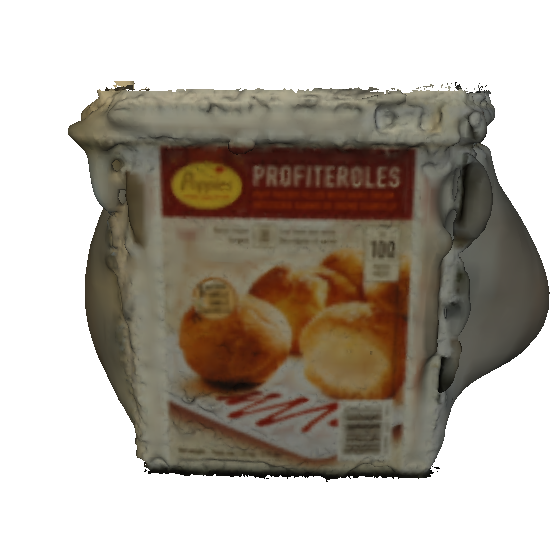
\includegraphics[width=0.2\textwidth]{interp/real_data/box/box_mvs}}&
\raisebox{-.5\height}{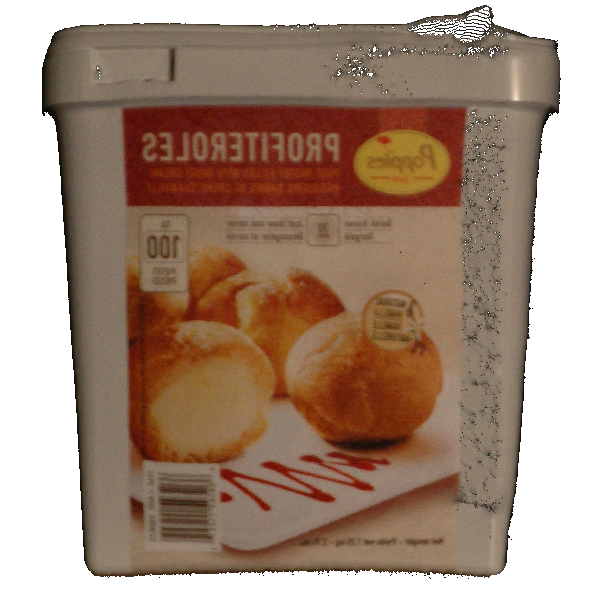
\includegraphics[width=0.2\textwidth]{interp/real_data/box/box_ps}}&
\raisebox{-.5\height}{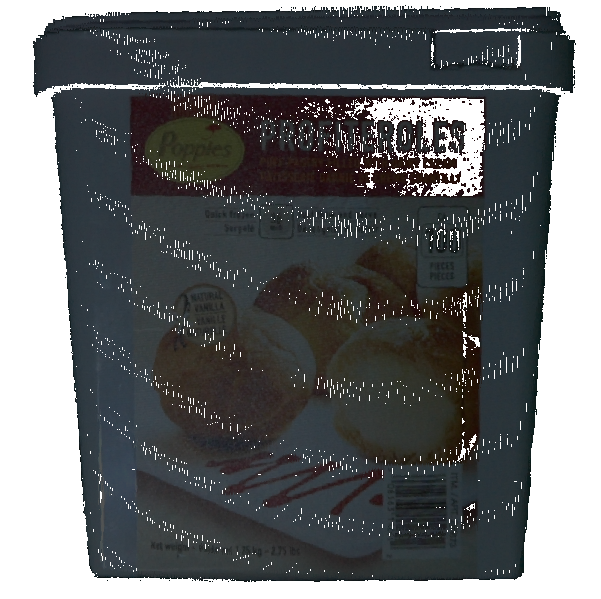
\includegraphics[width=0.2\textwidth]{interp/real_data/box/box_sl}}&
MVS, SL, PS\\
cat0 &
\raisebox{-.5\height}{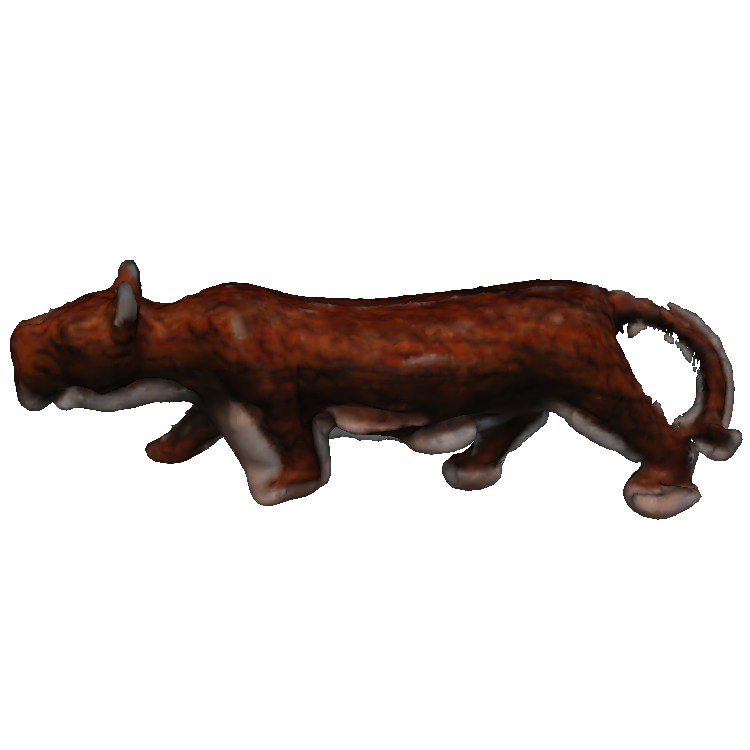
\includegraphics[width=0.2\textwidth]{interp/real_data/cat0/cat0_mvs}}&
\raisebox{-.5\height}{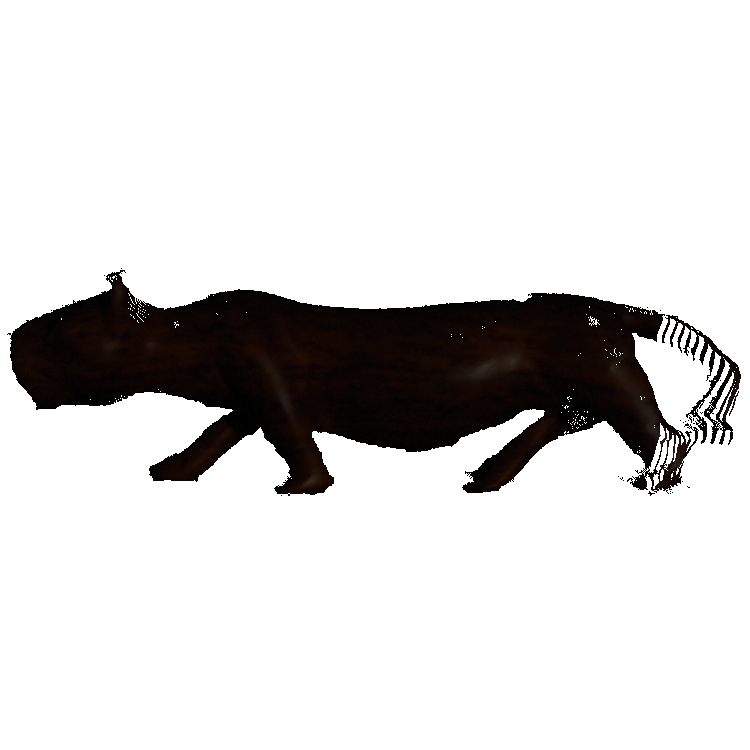
\includegraphics[width=0.2\textwidth]{interp/real_data/cat0/cat0_ps}}&
\raisebox{-.5\height}{
\includegraphics[width=0.2\textwidth]{interp/real_data/cat0/cat0_sl}}&
None\\
cat1 &
\raisebox{-.5\height}{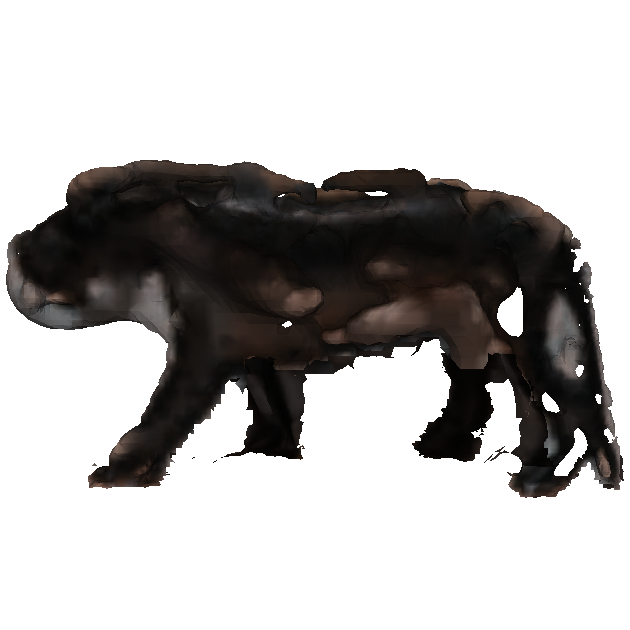
\includegraphics[width=0.2\textwidth]{interp/real_data/cat1/cat1_mvs}}&
\raisebox{-.5\height}{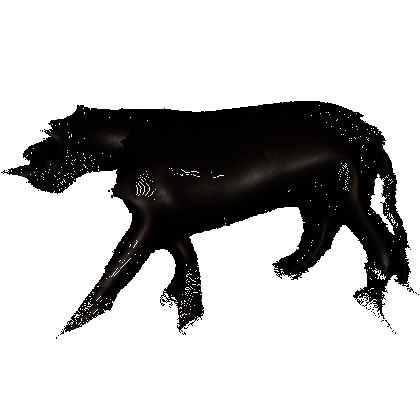
\includegraphics[width=0.2\textwidth]{interp/real_data/cat1/cat1_ps}}&
\raisebox{-.5\height}{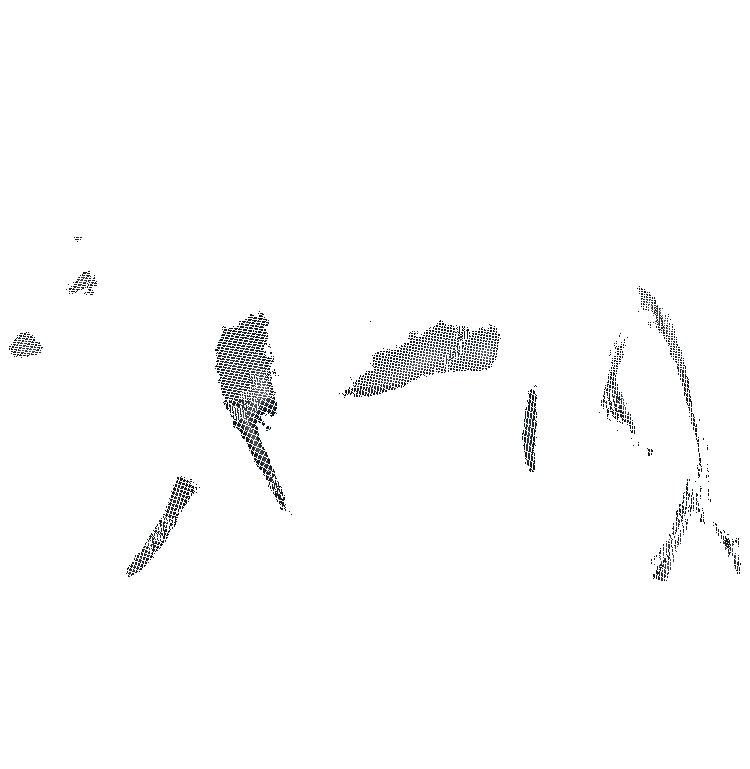
\includegraphics[width=0.2\textwidth]{interp/real_data/cat1/cat1_sl}}&
None\\
dino &
\raisebox{-.5\height}{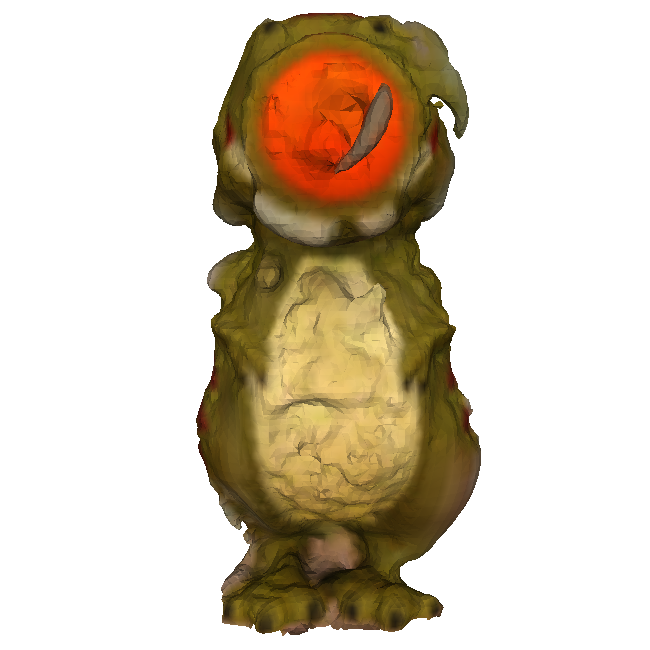
\includegraphics[width=0.2\textwidth]{interp/real_data/dino/dino_mvs}}&
\raisebox{-.5\height}{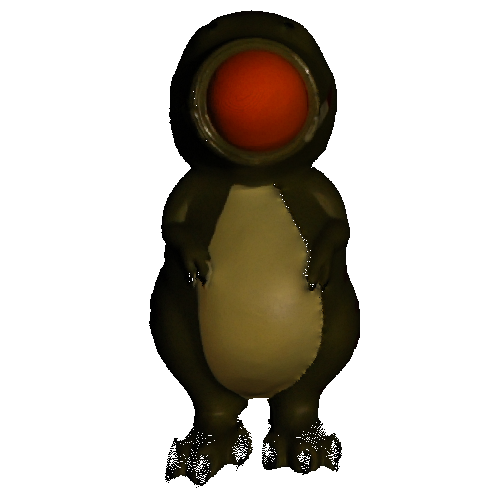
\includegraphics[width=0.2\textwidth]{interp/real_data/dino/dino_ps}}&
\raisebox{-.5\height}{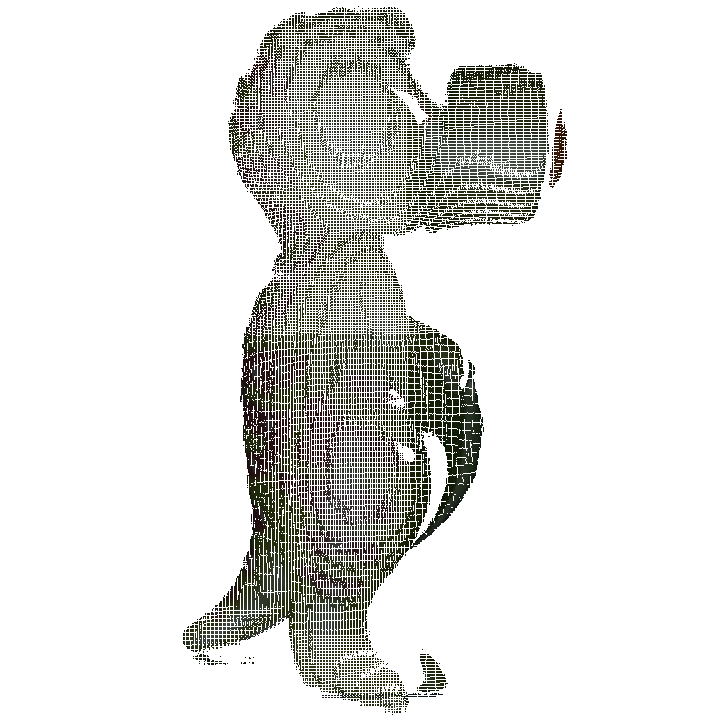
\includegraphics[width=0.2\textwidth]{interp/real_data/dino/dino_sl}}&
PS, SL\\
cup &
\raisebox{-.5\height}{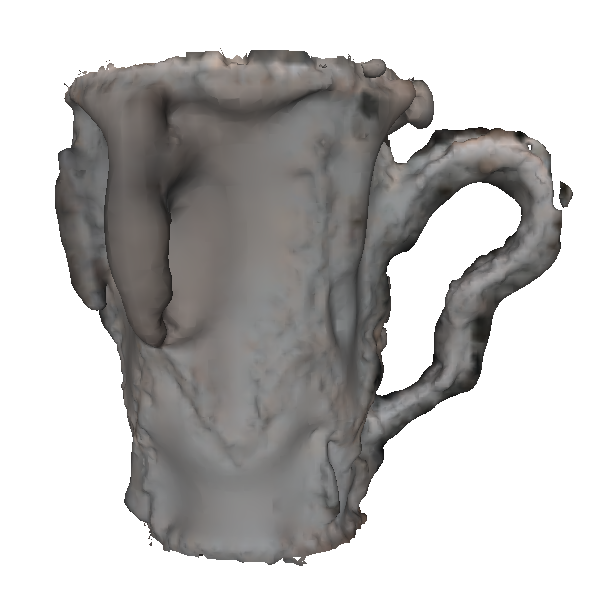
\includegraphics[width=0.2\textwidth]{interp/real_data/cup/cup_mvs}}&
\raisebox{-.5\height}{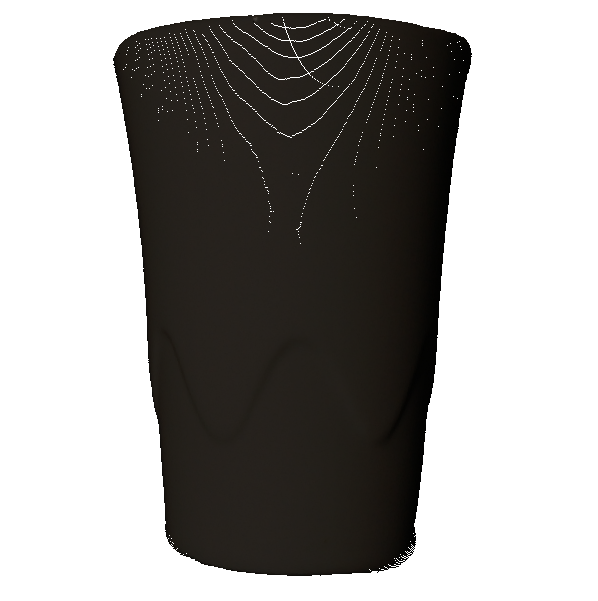
\includegraphics[width=0.2\textwidth]{interp/real_data/cup/cup_ps}}&
\raisebox{-.5\height}{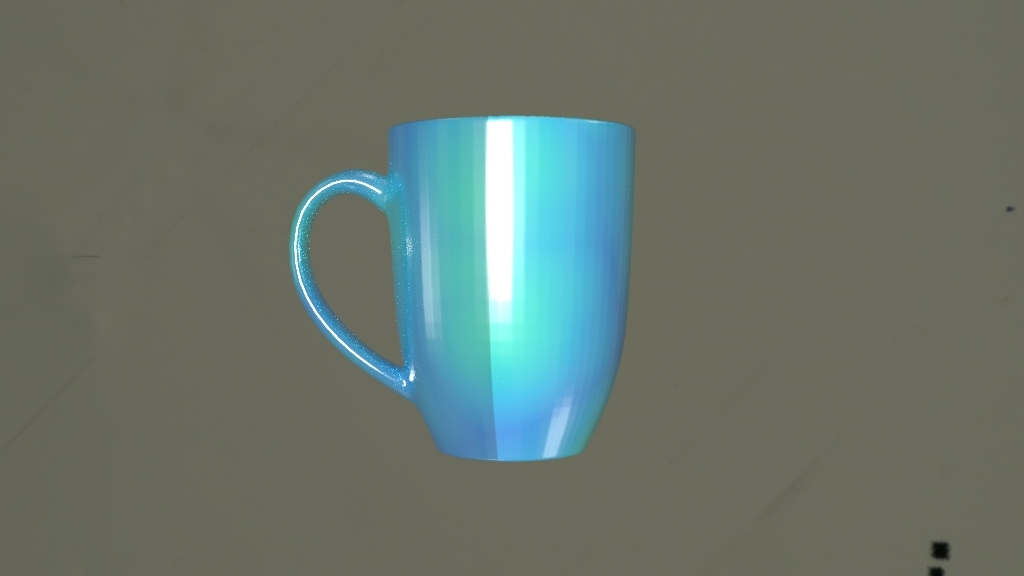
\includegraphics[width=0.2\textwidth]{interp/real_data/cup/cup_sl}}&
PS, SL\\
house &
\raisebox{-.5\height}{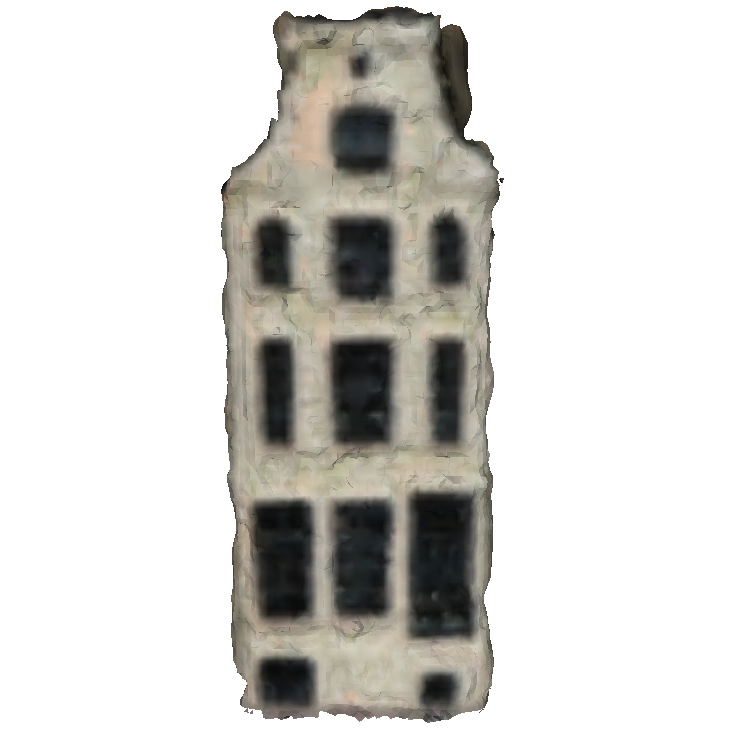
\includegraphics[width=0.2\textwidth]{interp/real_data/house/house_mvs}}&
\raisebox{-.5\height}{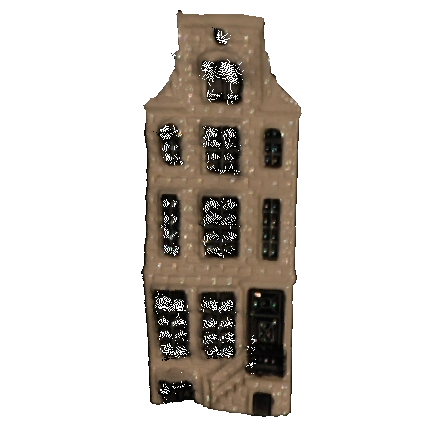
\includegraphics[width=0.2\textwidth]{interp/real_data/house/house_ps}}&
\raisebox{-.5\height}{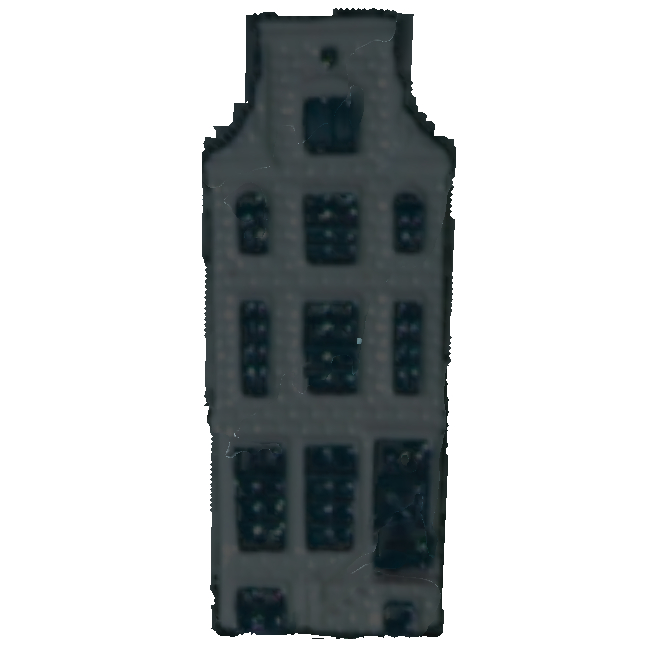
\includegraphics[width=0.2\textwidth]{interp/real_data/house/house_sl}}&
MVS\\
pot &
\raisebox{-.5\height}{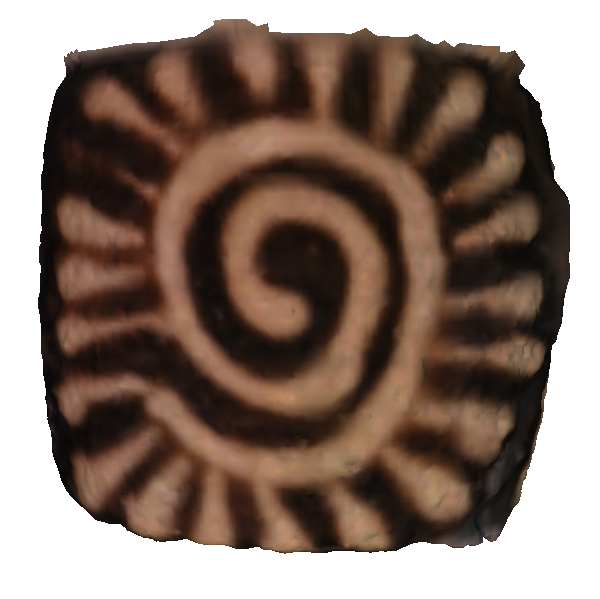
\includegraphics[width=0.2\textwidth]{interp/real_data/pot/pot_mvs}}&
\raisebox{-.5\height}{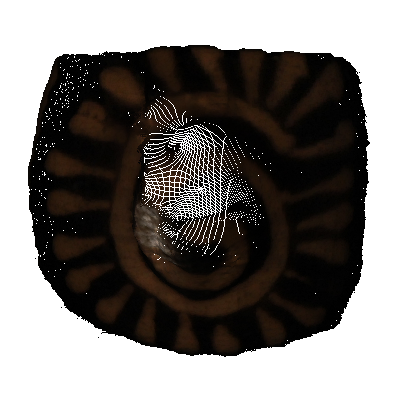
\includegraphics[width=0.2\textwidth]{interp/real_data/pot/pot_ps}}&
\raisebox{-.5\height}{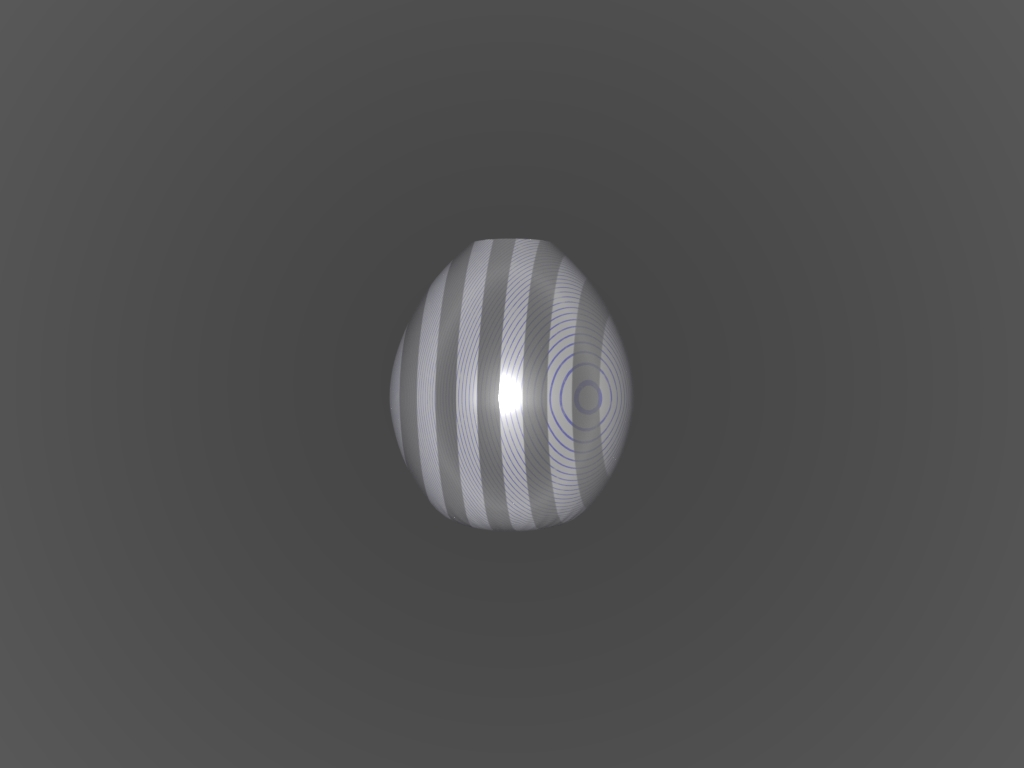
\includegraphics[width=0.2\textwidth]{interp/real_data/pot/pot_sl}}&
MVS, SL\\
\end{tabular}
\caption{Reconstruction results of MVS, PS, SL}
\label{fig:test_real_world_obj}
\end{figure}

\begin{figure}[h!]
\centering
\begin{tabular}{lcccr}
Object & PMVS & Example-based PS & Gray SL & Best-suited Algo.\\
statue &
\raisebox{-.5\height}{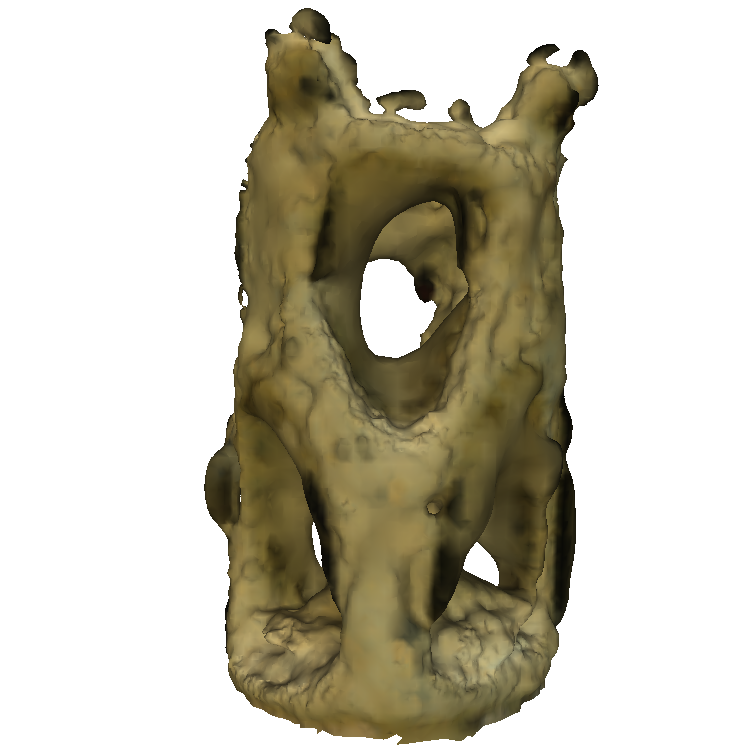
\includegraphics[width=0.2\textwidth]{interp/real_data/statue/statue_mvs}}&
\raisebox{-.5\height}{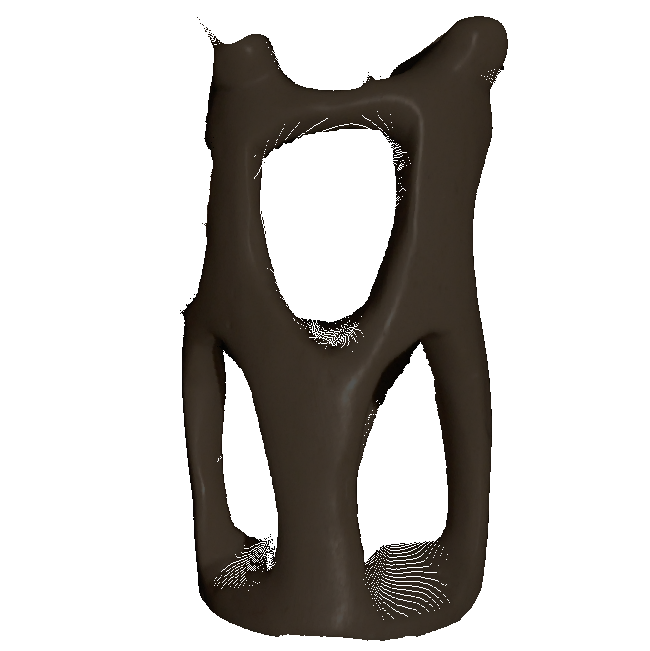
\includegraphics[width=0.2\textwidth]{interp/real_data/statue/statue_ps}}&
\raisebox{-.5\height}{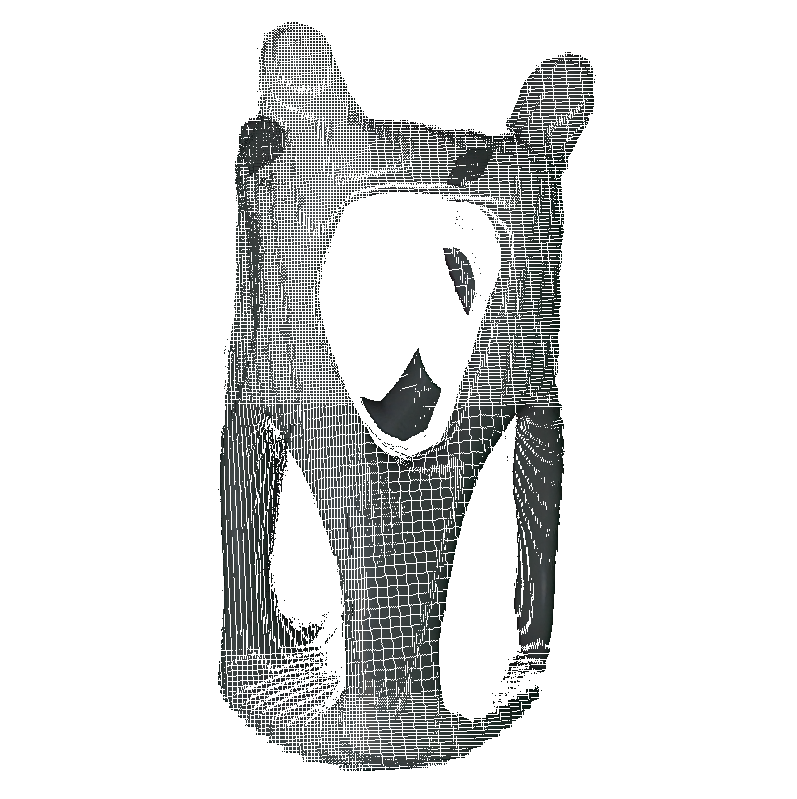
\includegraphics[width=0.2\textwidth]{interp/real_data/statue/statue_sl}}&
PS, SL\\
vase &
\raisebox{-.5\height}{\includegraphics[width=0.2\textwidth]{interp/real_data/vase/vase_mvs}}&
\raisebox{-.5\height}{\includegraphics[width=0.2\textwidth]{interp/real_data/vase/vase_ps}}&
\raisebox{-.5\height}{\includegraphics[width=0.2\textwidth]{interp/real_data/vase/vase_sl}}&
MVS\\
\end{tabular}
\caption{Reconstruction results of MVS, PS, SL (cont'd)}
\label{fig:test_real_world_obj}
\end{figure}